\chapter[Eigene "Uberlegungen und die Implementierung \anmerkung{30 Seiten }]{Eigene "Uberlegungen und die Implementierung der resultierenden L"osung
\normalsize{Die Java-Applikation, Die Secondo Algebra, Experimante mit Regionen \anmerkung{30-40 Seiten }}
}
\minitoc
\newpage
\section{Vor"uberlegungen \anmerkung{7 Seiten}} \label{vorueberlegungen}
Im folgenden werde ich die Vorschl"age aus der Literatur, die ich oben beschrieben habe, bewerten und einige Gedanken ausführen, die ich mir zum Theme Matching gemacht habe. Ausserdem gebe ich an, welche dieser Vorschläge ich verwirklicht habe, und welche noch auf ihre Implementierung warten.

\subsection[Bewertung der Vorschl"age aus \cite{TG}]{Bewertung der Vorschl"age aus ,,Creating Repesentations for Continuously Moving Regions from Observations''\cite{TG}}
\begin{enumerate}
\item Position of centroid\index{Match!Schwerpunkt}

In dem Paper wurde diese M"oglichkeit nicht weiter betrachtet, da die Autoren davon ausgehen, dass ein Referenzpunkt, der auch au"serhalb des Polygons liegen kann nicht zu guten Matchings f"uhren kann. Hierzu muss angemerkt werden, dass im Rahmen der vorliegenden Arbeit das Matching auf Ebene des ConvexHullTrees durchgef"uhrt wird, und lediglich mit konvexen H"ullen von Polygone gearbeitet wird. Der Schwerpunkt einer konvexen H"ulle liegt nat"urlich aber wieder innerhalb dieser (wenngleich nicht zwangsl"aufig auch innerhalb des repr"asentierten Polygons). Au"serdem erscheint es plausibel, dass ein Referenzpunkt-Verfahren seine St"arke gerade dort haben wird, wo die "Uberlappungsalgorithmen ihre Schw"achen haben (bei sich schnell bewegenden, kleinen Objekten).

\begin{figure}
	\centering
	
\includegraphics{feu_logo2.eps}
	\caption[Beispiel für den Vorteil von Referenzpunktverfahren]{Beispiel für viele kleine Flächen, die sich relativ schnell bewegen. Wie man sehen kann, würde ein Überlappungsverfahren hier kein einziges Match, Referenzpunktverfahren aber eventuell alle möglichen finden.}
	\label{fig:SchnelleBewegung}
\end{figure}


Ausserdem ermutigte mich die Arbeit \cite{AFRW} darin diesen Ansatz weiterzuverfolgen.

Der Vorschlag, "`N"achste Nachbarn"' zu benutzen, hat den Nachteil, dass man so nur 1:1 Matches finden kann. Im Rahmen der vorliegenden Arbeit wurde stattdessen Schwellwert-Verfahren gew"ahlt. Siehe hierzu \ref{Schwellwert}.

\item Fixend threshold (set of cycles)\item{Match!Überlappung}

Das Verfahren wurde analog zur Beschreibung Erlend T\o{}ssebros "ubernommen und implementiert. 

Klar ist, dass dieses Verfahren dann Schwächen aufweisen wird, wenn sich kleine Flächen so stark bewegen, dass diese sich nicht mehr, oder nur noch wenig überlappen. Bei kompliziert aufgebauten Flächen, die sich relativ wenig bewegen wird dieses Verfahren aber den Vorteil aufweisen, dass relativ wenige falsche Flächen gematcht werden.

\begin{figure}
	\centering
	
\includegraphics{feu_logo2.eps}
	\caption[Beispiel für den Vorteil des Overlaping-Match]{Beispiel eine Matches von komplitzierten Regionen. Wie man sehen kann, würde ein Überlappungsmatch nur die richtigen Übereinstimmungen zurückgeben, ein Referenzpunktverfahren aber deutlich mehr.}
	\label{fig:OverlapVorteil}
\end{figure}


\item Maximize Overlap (set of cycles)

Dieses Verfahren k"onnte interesannt sein, da es mir aber im  Rahmen dieser Arbeit nicht möglich ist alle interesannten Matches zu implementieren, habe ich auf die Implementierung dieses Matches verzichtet.

\end{enumerate}

\subsection[Bewertung der Vorschl"age aus \cite{AAR}]{Bewertung der Vorschl"age aus ,,Matching Shapes with a Reference Point'' \cite{AAR}}

Wie ich unter \ref{BedeutungAAR} bereits ausgeführt habe, habe ich den Algorithmus $S$, den allgemeinsten aus dieser Arbeit, nicht implementiert. Die Idee ein Match auf Basis des Steinerpunktes zu implementieren brachte mich dazu, einen Match zu implementieren, dass simultan zu dem Verfahren ,,Position of centroid'' aus \cite{TG} funktioniert, aber den Steinerpunkt als Referenzpunkt benutzt.

\subsection[Bewertung der Vorschl"age aus \cite{AFRW}]{Bewertung der Vorschl"age aus ,,Matching Convex Shapes with Respect to Symmetric Difference'' \cite{AFRW}}

Es gilt im Wesentlichen das Selbe, dass ich schon im letzten Absatz sagte. Ich habe den Algorithmus aus der Arbeit nicht imlementiert, aber ich habe die beiden Verfahren ,,Fixend threshold'' und ,,Position of centroid'' aus \cite{TG} implementiert. Wie ich unter \ref{BedeutungAFRW} ausführe weisen beide Verfahren  eine gewisse Verwandschaft zu dem einfachsten Algorithmus dieser Arbeit auf. 


\subsection{\index{Match!Refenrzpunkt}Matching mit Referenzpunkten}

Die meisten Matching-Verfahren basieren auf Referenzpunkten. Unter \ref{AARR} und \ref{AFRWW} wurden Verfahren angegeben, die zu bestimmten Referenzpunkten Matchings mit garantierter Qualität liefern. Ich habe mir einige Gedanken gemacht, wie man Referenzpunktverfahren im Allgemeinen durchführen könnte.

\subsubsection*{statistische Analyse}

Zunächst kann man ein Feld aufgebauen, in dem zu jeder Kombination von Cycles die Entfernung der Referenzpunkte eingetragen wird. Sortiert man dieses Feld aufsteigend nach den Entfernungen, so steht zu erwarten, dass es zwischen den erwünschten und den unerwünschten Beziehungen einen Sprung in dem Graphen geben wird.  Diesen Sprung m"u"ste mit geeigneten statistischen Verfahren bestimmt werden werden k"onnen. 

Nachteilig an diesem Verfahren ist, dass die Laufzeit dieses Verfahrens hoch ist. Finden sich auf den beiden Seiten des Matchings $n$ beziehungsweise $m$ Referenzpunkte, so hat das resultierende Feld die Dimension $n\times m$. Dieses Feld kann in $O(n\times m)$aufgebaut werden. Zum Sortieren des Feldes wird dann $O((n\times m)\log(n\times m))$ verwendet. Also ist dieses Verfahren mindestens vom Typ $O((n\times m)\log(n\times m))$ (je nach dem verwendeten statistischen Verfahren k"onnte die Laufzeit sogar schlechter sein).

Aufgrund der oben benannten schlechten Laufzeit und unter dem Aspekt, dass kein geeignetes Verfahren zur Verfügung steht, wird in der vorliegenden Arbeit diesem Ansatz keine weitere Beachtung geschenkt. Eine weitere Betrachtung dieses Verfahrens könnte dennoch interesannt sein.

\begin{figure}
	\centering
	
\includegraphics{feu_logo2.eps}
	\caption[Beispiel für eine statistische Analyse]{Beispiel für den Grapfen aller Entfernungslängen eines Matches mit eingezeichneter Schwelle}
	\label{fig:statistik}
\end{figure}


\subsubsection*{\index{Match!Schwellwert}Schwellwertverfahren}\label{Schwellwert}

Das Schwellwertverfahren kann wie folgt formuliert kann: ,,Matche zwei Cycle, wenn der Abstand ihrer Referenzpunkte kleiner als der Schwellwert ist.''

Die Laufzeit dieses Verfahrens ist wesentlich besser. Zu jedem der $m\times n$ verschiedenen  Referenzpunkte wird der  Abstand (in konstanter Zeit) berechnet und mit dem Schwellwert vergleichen. Also ist die Laufzeit$O(m\times n)$.

Aufgrund der Verschiedenheit der m"oglichen Daten ist ein solcher absoluter Schwellwert $t_{abs}$ nat"urlich nicht handhabbar, so dass die Matchingfunktion mit einem relativen Schwellwert $t_{rel}$ (in \%) arbeiten muss. Aus diesem wird dann intern ein absoluter Schwellwert berechnet, der dann wie oben verwendet wird. Man berechnent $t_{abs}$, indem man $t_{rel}$ mit dem gr"o"sten Abstand multipliziert, den die beiden Regionen voneinander haben. Leider ben"otigt man f"ur die Berechnung dieses Wertes $O(n\times m)$. Praktisch wird desshalb ein Algorithmus verwendet, der in $O((n+m)\log{n+m})$ einen sehr "ahnlich Wert berechnet. Siehe hierzu \ref{maxDist}.

\subsubsection*{neuronale Netze}

Man kann die Problematik, Matches von Referenzpunkten zu finden auch wie folgt beschreiben. In einer Menge von Punkten im $\mathbb{R}^2$ werden Klassen von zusammengehörigen Punkten gesucht.

Solche Klassifizierungsaufgaben sind genau das klassische Einsatzgebiet von neuronalen Netzen. Es steht zu erwarten, dass ein Lernverfahren auf Basis von neuronalen Netzen sehr gute Ergebnisse liefern wird. Der Rahmen dieser Arbeit würde aber von einem solchen deutlich überschritten.

\subsection{Beseitigung von 1:n Matches}\label{1zuN}

Der Algorithmes, welcher aus dem Match movingSegments erzeugt, kann ausschließlich mit Matches umgehen, wo es zu jedem Source maximal ein Target gibt. Taucht ein 1:n Matching auf, dann muss diese also aufgel"ost werden. 

\subsubsection*{Alle $n$ Targets sind Kinder einer einzigen ConvexHullTreeNode}\label{JoinConc}

Sind alle $n$ Targets Kinder einer einzigen ConvexHullTreeNode, so gibt es einen Algorithmus, der schon in \cite{TG} beschrieben wurde. Kurz gesagt geht es darum, die konvexe H"ulle aller Targets zu bilden, und das Matching von den $n$ Targets auf diese neue H"ulle umzuleiten.

Leider versagt dieses Verfahren, falls die gematchten Polygone sich nicht ähnlich genug sind. Es gelang mir nicht, genau zu analysieren, in welchen Fällen genau die Probleme auftauchen. Deshalb musste ich auf die Implementierung dieses Verfahrens verzichten. Falls das Verfahren funktionierte, sahen die Ergebnisse aber sehr gut aus. Es erscheit daher lohnenswert diesem Verfahren weiter nachzugehen.

\subsubsection*{Source ist ein Face, oder ein Hole}

Ist die Source ein Face, oder ein Hole,  so muss versucht werden den Source aufzuteilen. Ich habe einige Überlegungen angestellt, wie es möglich ist diese Zerteilung möglichst schonend, will meinen ohne das man das zu teilende Objekt und alle Matches von diesem neu berechen muss, vornahmen kann.
\begin{itemize}
\item Eine ConvexHullTreeNode ist nur an Eckpunkten, oder an Punkten auf Linien zu teilen, die keine Kinder haben, da sonst die ConvexHullTree zerst"ort w"urden.

\item Eine ConvexHullTreeNode ist nur an zwei Punkten zu teilen, wenn das beschriebene Polygon auch nur in zwei Teile zerf"allt.

\item Die Zerteilung der Source-Komponente sollte die Lage und das Verh"altnis der Fl"acheninhalte der Target-Komponenten weitestgehend wiederspiegeln.

\end{itemize} 

Nach Rücksprache mit Herr Professor Ralf Hartmut G"uting habe ich diesen schonenden Ansatz nicht weiterverfolgt, sondern ein Verfahren gefunden, dass bei dem Zerteilen schönere Ergebnisse findet. Der Preis davon ist, dass die erzeugten Objekte und alle Matches dieses Objekten komplett neu berechnet werden müssen. Bei der Neuberechnung der neuen Matches ist zu beachten, dass man hier in keine Endlosschleife laufen darf. So eine Endlosschleife kann entstehen, wie das folgende Beispiel zeigt.

Nehmen wir an, dass das Polygon $A$ gegen zwei Polygone $B_1$ und $B_2$ gematcht wird. Deshalb wird $A$ in $A_1$ und $A_2$ geteilt. Bei der Neuberechnung des Matches wird nun $A_1$ wieder gegen $B_1$  und $B_2$ gematcht. Also muß $A_1$ in $A_{1_1}$ und $A_{1_2}$ geteilt werden, die leider wieder gegen $B_1$ und $B_2$ gematcht werden. ...

Um solche Effekte zu umgehen, darf man für $A_1, A_2,B_1$ und $B_2$ nicht ein normales Match berechen, sonden man darf $A_1$ und $A_2$ nur gegen das eine $B_i$ matchen, das am besten passt. 

Wird in Face zerteilt, so kann es passieren, daß ein Hole zerteilt werden. Falls sich das nicht verhindern l"asst, so zerf"allt das Loch in zwei neue Konkavit"aten, die den neuen Faces hinzugefügt werden müssen. Ein Algorithmus der dieses Leistet findet sich unter \ref{JoinLL} Nichtzerteilte Holes müssen demjenigen neuen Face zugeordnet werden, in dem diese liegen.

Um ein optisch möglichst ansprechendes Resultat zu erzeugen, müssen sich Form und Lage der Targetobjekte in der Aufsplittung wiederfinden. Ein Algortihmus der dieses liefert findet sich unter \ref{ZerteilungsAlgo}. Bei diesem Algorithmus gehen nur zwei Polygone auf der Targetseite in die Zerteilung ein. Weitergehende Zersplitterungen lassen sich durch die mehrfache Anwendung dieses Algorithmusses erzeugen.

\subsubsection*{Source ist ein untergeorneter ConvexHullTreeNode}

Da man in diesem Fall das oben beschriebene Verfahren nicht anwenden kann, muss man auf folgenden, sehr einfachen Algorithmus zurückgreifen, der analog zu dem Verfahren funktioneiert, mit welchem im letzen Abschnitt Endlosschleifen vermieden wurden:

Wird $A$ auf  $B_1,B_2, \hdots ,B_n$ gematcht, so lösche alle Matches, außer dem einen, welches die höchste Bewertung aus allen Einzelmatches von $A$ auf $B_i$ hat.

Obwohl dieses Verfahren sehr einfach ist, sehen die Ergebnisse überraschen gut aus. Eine Verbesserung könnte hier allenfalls duch den Algorithmus von T\o{}ssebro erreicht werden, wenn man dessen unerwünschte Verhalten abstellen könnte.

\subsection{Beseitigung von "`gedrehten Konkavit"aten"'}\label{gedrehtKon}
In manchen F"allen versagt das in \cite{TG} genannte Verfahren, um aus Matchings Moving-Regions zu erzeugen. Dieses, in Kapitel "`6 Interpolating between two arbitray polygones"' beschriebene Verfahren setzt voraus, dass die beiden gematchten Kinderpolygone ein gemeinsames, aus zwei Dreiecken zusammengesetztes Trapez in der Aussenh"ulle der beider Vaterpolygone besitzen. 

Dies ist zum Beispiel dann nicht der Fall, wenn wir uns als Quellpolygon ein "`U"', und als Zielpolygon ein um 90$\degree$ gedrehtes "`U"' vorstellen. Auch wenn die Konkativit"aten richtig zueinander gematcht sind, versagt das bekannte Verfahren.

Die, das Matching abschlie"sende, Funktion kann solche F"alle erkenne, indem es die Winkel betrachtet, die die gemeinsame Kante von Kind und Vater, sowie die beiden Nachbarkanten des Vaters, mit der x"-Achse haben. Ist der Winkel der gemeinsamen Kante auf der einen Seite nicht im  Intervall der Winkel der Nachbarkanten der anderen Seite, so liegt der Fall vor, dass das Verfahren nicht funktioniert.

\begin{figure}
	\centering
	
\includegraphics{feu_logo2.eps}
	\caption[Beispiel für gedrehte Polygone]{Beispiel für gedrehte Polygone bei denen das ,,rotating pane'' Vefahren versagt, da die Öffnungen der Konkativitäten kein Trapez bilden.}
	\label{fig:gedrehteMatches}
\end{figure}


Wenn ein solcher Fall erkannt wird, so gibt es zwei M"oglichkeiten zu reagieren:
\begin{itemize}
\item Beide Konkativit"aten werden gegen $null$ gematcht

In diesem Fall verschwindet die Konkativit"at auf der einen Seite  und zeitgleich entsteht auf der anderen Seite eine Neue. Obwohl dieses Verfahren das deutlich Einfachere ist, zeigt sich in der praktischen Anwendung, dass das Resultat den Erwartungen weitestgehend entspricht.

\item Die beiden Konkativit"aten werden zu L"ochern umgewandelt

In diesem Fall werden beide Konkavit"aten in L"ocher verwandelt, die dann zueinander gematcht werden. Im Resultat w"urde sich die Konkativit"at von der einen Seite abl"osen, und zu der anderen Seite wandern. M"oglicherweise sieht dieses Verfahren nat"urlicher aus, es ist aber nicht absehbar, was passiert, wenn der Weg zwischen den beiden Positionen nicht "`frei"' ist (etwa weil sich hier ein weiteres Loch oder eine Konkativit"at befindet). Aus diesen Gründen habe ich mich für die Implementierung des ersten Verfahrrens entschieden.
\begin{figure}
	\centering
	
\includegraphics{feu_logo2.eps}
	\caption[Schnappschüsse von den gedrehten Polygonen]{Zwei Schnappschüsse von dem Match aus Abbildung~\ref{fig:gedrehteMatches}, in dem die Konkativitäten gegen $null$ gematcht wurden.}
	\label{fig:gedrehteMatches2}
\end{figure}

\end{itemize}


\subsection{\index{Match!optimales}Erstellung eines Matchings aus mehreren Anderen}\label{bewertung}


Es ist festzustellen, das unter der Betrachtung der bereits erstellten Matchings, dass das Overlapping-Match besser auf Vereinigungen und Aufsplitterungen von Cycles reagiert, und dass das Schwerpunkt-Verfahren besser auf kleine und schnelle Cycles abgestimmt ist. 

Es scheint also ein verfolgenswerter Ansatz zu sein, beide Matches (und vielleicht noch andere, etwa Overlapping mit mehreren Schwellwerten), zu berechnen, und aus diesen das beste Matching zu bestimmen. 

Zur Bestimung der G"ute eines gegebenen Matchings sind folgende Verfahren angedacht. Damit die verschiedenen Bewertungen vergleichbar sind, sind diese auf 1 normiert.

\begin{itemize}
\item Die \index{Bewertung!Overlap}Overlap-Bewertung: 

Ein gro"ser Durchschnitt der "Uberlappungen wirkt sich positiv auf die Bewertung aus.

Dieses Bewertungsverfahren korrespondiert zwar direkt mit dem Overlaping-Match wird aber trotzdem in dieser Arbeit benutzt, da die Überlappung sich als sehr interesanntes Kriterium erwiesen hat. Die Berechnung l"auft so:

$$r_O=\frac{\sum_{m\in M} \frac{A_{overlap}}{A_{source}+A_{target}}}{|M|}$$

\item Die \index{Bewertung!Hausdorff}Hausdorff-Bewertung:

In \cite{AAR} wird die,  oben bereits eingef"uhrte, Hausdorff-Norm benutzt, um Matchings zu bewerten. 

Bei der Implementierung dieser Norm stellt sich die Frage der Normierung. Mangels Alternative habe ich mich dazu entschlossen, alle einzelnen Hausdorff--Abst"ande duch den Duchmesser $d$ der Ausgangsregionen zu teilen.  Durchmesser bezeichne hierbei den Gr"o"sten Abstand, den zwei Punkte zueinander haben. Dieses Vorgehen bedeutet aber leider, dass die Abst"ande von kleinen Konkavit"aten relativ wenig in die Gesamtbewertung eingehen. Die Berechnung lautet:

$$r_H=\frac{\sum_{m\in M}\delta_H(m)}{|M|\times d}$$

\item Bewertung durch Minimierung einer Norm duch geeignete Abbildungen

\cite{AAR} und \cite{AFRW} enthalten beide die Bewertung:
$$\min_{T\in\mathcal{T}}\delta(A,T(B))$$
$\delta$ kann hierbei entweder der Hausdorff-Abstand oder die symetrische Differenz sein. Das Problem an diesem Ansatz ist die Berechnung der minimierenden Abbildung $T$. Algorithmen zur Findung dieser Abbildung werden zwar angegeben, die Implementierung dieser würden aber den Umfang dieser Arbeit sprengen.

\item Die \index{Bewertung!Referenzpunkt}Referenzpunkt-Bewertung:

Ein kleiner Durchschnitt der Entfernungen der zueinander gematchten Referenzpunkte wirkt sich positiv auf die Bewertung aus.

Da dieses Verfahren direkt mit dem Schwerpunkt-Match, bzw. dem Steinerpunkt"=Match korrespondiert, und ausserdem nach \cite{AFRW} und \cite{AAR} nicht zu erwarten steht, dass dieses Verfahren deutlich andere Werte als die Overlap-Bewertung, bzw. die Hausdorf-Bewertung liefert, verfolge ich dieses nicht weiter.

\item Die \index{Bewertung!Flächensummen}Summen-Bewertung:


Etwa gleich gro"se, zueinander gematchte Fl"achen, wirken sich positiv auf die Bewertung aus.

Es steht zu erwarten, dass zueinander geh"orige F"achen etwa gleich gross sind. Auch wenn sich eine Fl"ache in mehrere andere teilt, wird die Summe der Fl"acheninhalte in etwa so gro"s sein, wie der Fl"acheninhalt der Ursprungsfl"ache. Zur Normierung teile ich den Kleineren durch den gr"o"seren Fl"acheninhalt, und bekomme somit die Abweichung in Prozent. Die Berechnung l"auft so:

$$A_{target}=\sum_{t\in Target}A_t$$
$$r_A=\frac {\sum_{m\in M}\frac{\min{A_{source},A_{target}}}{\max{A_{source},A_{target}}}}{|M|}$$



\item Die \index{Bewertung!linear}Linear-Bewertung

Bei der Implementierung der obigen Verfahren zeigte sich, dass die Verfahren eine Tendenz zu "ubertriebenen Zersplitterungen aufweisen. Unter der Pr"amisse, dass dies in den allermeisten F"allen eher unerwünscht ist, f"urte ich diesen Bewertungsfaktor ein, um dieses Verhalten abzuschw"achen.

F"uhrt das Matching zu einer geringen Anzahl an Zersplitterungen, so wirkt sich das positiv auf die Bewertung aus.

Die Berechnung l"auft so:

$$L(m)=
\begin{cases}
	\frac{1}{2} & \text{falls }|targets|=0\\
	\frac{1}{|targets|} & \text{sonst}
    \end{cases}
$$

$$r_L=\frac{\sum_{m\in M}L(m)}{|M|}$$

\item Die \index{Bewertung!strukturell}Struktur-Norm:

Stimmen die aufeinander gematchten Cycles strukturell weit "uberein, so wirkt sich das positiv auf die Bewertung aus (eventuell kann man hier die Struktur der jeweiligen ConvexHullTrees heranziehen).

Diese Norm finde ich nach wie vor interesant, habe sie aber noch nicht weiter verfolgt. Zur Struktur der ConvexHullTrees ist zu sagen, dass in \cite{TG} der Umstand beschrieben ist , das "ahnliche Polygone teilweise recht unterschiedliche ConvexHullTree-Repr"asentationen aufweisen k"onnen, was eine solche Bewertung nat"urlich negativ beweinflussen kann\footnote{Dieses ist aber weniger schlimm als es klingt, Herr T\o{}ssebro macht in diesem Artikel plausiebel, dass dieses Problem eher ein Problem von kleinen, k"unstlichen Testdatens"atzen als von realen Daten ist}.


\end{itemize} 

Wie man am Beispiel der Summen-Norm sehen kann, gibt es mehr M"oglichkeiten zu bewerten, als es effiziente Matchings gibt. Das Summen-Matching, das lauten k"onnte: "`Matche ein Cycle mit  einer Menge von Anderen, wenn die Summe der Fl"acheninhalte fast gleich ist zu dem Fl"acheninhalt des einen Cycles"', entspricht dem Rucksack-Problem und ist daher nicht effizient l"osbar. Die Bewertung, wie gut ein gegebenes Matching ist, ist mit diesem Verfahren aber effizient m"oglich.

\section{Gemeinsame Grundlagen \anmerkung{20 Seiten}}

\subsection{Beschreibung von verwendeten Algorithmen} \label{Algorithmen}
In disem Abschnitt werde ich Algorithmen vorstellen, die entweder sehr zentral f"ur die L"osung des Interpolationsproblems sind, oder Algorithmen, die keine Standard-Algorithemen sind. Diese Algorithmen musste ich also selbst entwickeln.

\subsubsection{\index{Hashwerte!Berechnung}effiziente Berechnung von Hashwerten aus RegionTreeNodes}\label{berechenHashwerte}

Um RegionTrees als Schlüssel in der Hash-Table benutzen zu können muß aus diesen ein Hashwert berechnet werden können. In die Berechnung des Hashwertes muss jede einzelne Ecke des RegionTrees eingehen. Damit ist die Ermittelung dieses Wertes leider eine recht aufwendige Operation, zumal auf diesen Wert im Verlauf eines Matching-Verfahrens sehr oft zugegriffen werden muss. Desshalb ist es nötig, die Hashwerte dieser Objekte zu cachen. 

Um sicherzustellen, dass ein Hashwert immer aktuell ist und keine überflüssigen Neuberechnungen notwendig sind habe ich ein Chachingverfahern gewählt, dass analog zu einem bekannten Verfahren aus der technischen Informatik abläuft. Jedes Objekt des RegionTrees verfügt über ein ,,Dirty-Flag''. Dieses Flag gibt an, ob der gecachte Wert noch aktuell ist. Dieses Flag wird bei jeder Operation gesetzt, die das Objekt so verändert, dass sich der Hashwert auch ändern müsste. Bei jedem lesenden Zugriff auf den Hashwert wird 
\begin{itemize}
\item der gecachte Wert zurückgegeben, falls das Dirty-Flag nicht gesetzt ist,
\item ist das Dirty-Flag gesetzt, so wird der Hashwert neu berechnet, das Dirty-Flag gelöscht und der neuberechnete Wert gelöscht.
\end{itemize}

Beim Setzen des Dirty-Flags ist darauf zu achten, dass auch bei dem Vaterelement und alle Vorfahren des Vaterelements dieses gesetz werden muss.

Dieses Verfahren stellt sicher, dass die Berechnung des Hashwertes wirklich nur dann erfolgt, wenn dies notwendig ist.

Die Berechnung geht wie folgt von statten:

\begin{itemize}
\item Konvexer Hüllenbaum

Die Berechnung startet mit einem zufällig  gewählten, fixen Wert. Zu diesem wird dann die kummulierte Summe gebildet, $HV=\lfloor HV+x_i*321+y_i*312\rfloor$. Die Zahl 312 ist wieder wilkürlich gewählt. Da sich aber Geographische Koordinaten oft nur wenig unterscheiden, und eine Unterscheidung etwa von Dreiecken, die nahe beieinander liegen gewährleistet sein muss, darf dieser Wert nicht zu klein gewählt sein. 

In die Berechnung gehen auch noch ein vielfaches des Levels und eine feste Zahl ein, die nur zum tragen kommt, falls das Objekt ein Hole ist.

\item Face

Der Wert für ein Face wird berechnet, indem man zu dem Hashwert des Cycles alle Hashwerte der Löcher hinzuaddiert. Dem Ergebnis wird noch ein weiterer konstanter Summand beigebracht. Somit ist sichergestellt, das der Hashwert eines Faces, welches nur aus einem einzigen Cycle besteht, sich von dem Hashwert des Cycles unterscheidet.

\item Region

Der Hashwert einer Region setzt sich wiederum aus den Hashwerten seiner Faces und einem weiteren konstanten Summanden zusammen.
\end{itemize}

\subsubsection{\index{splitline!Berechnung}Berechnung einer Zerlegungslinie für ein ConvexHullTreeNode aus zwei Anderen}\label{ZerteilungsAlgo}

Dieser Algorithmus bekommt ein zu zerteilendes ConvexHullTreeNode ($A$) und zwei andereConvexHullTreeNodes ($B_1$ und $B_2$). Berechnet werden soll nun ein Linienzug, der die Lage und Form von $B_1$ und $B_2$ möglichst gut wiedergeben soll, und an dem sich $A$ zerteilen lassen kann.

Die weitere Besprechung dieses Algorithmuses werde ich am Beispiel von drei Polygonen vornehmen. Diese Drei sind in Abbildung~\ref{fig:ZuZersplitten} zu sehen.

\begin{figure}
	\centering
	\includegraphics[scale=0.6]{ZuZersplitten.eps}
	\caption[Zu teilendes Polygon mit Referenzpolygonen]{Die Polygone $A$ (gelb), $B_1$ (blau) und $B_2$ (rot).}
	\label{fig:ZuZersplitten}
\end{figure}

Zuerst werden die Schwerpunkte $M_1$ und $M_2$  von $B_1$ und $B_2$ berechnet. Dann werden die Eckpunkte der beiden Polygone nach solchen Punkten gefiltert, die auf einer Orthogonalen zu der Strecke zwischen $M_1$ und $M_2$ liegen Die beiden Ergebnislisten werden nach dem Abstand von dem Punkt zu der Linie sortiert, wobei die Abstände auf einer Seite der Linie negativ gewertet werden.

Die beiden Listen der Endpunkte sehen für unser Beispiel au, wie folgende Tabellen. Abbildung~\ref{fig:RectDist} zeigt die ensprechenden Punkte.

\begin{tabular}{|c|r|r|r|r|r|r|r|r|}

\multicolumn{9}{c}{Die Punkte von $B_1$} \\
\hline
Punkt&
 102&
 103&
 104&
 106&
 105&
 107&
 108&
 109\\
\hline
Entfernung&
   88&
   44&
   35&
   16&
   -1&
  -29&
  -49&
 -111\\
\hline
\end{tabular} 

\begin{tabular}{|c|r|r|r|r|r|r|r|}


\multicolumn{8}{c}{Die Punkte von $B_2$} \\
\hline
Punkt&
 206&
 205&
 204&
 203&
 202&
 201&
 200
\\
\hline
Entfernung&
   75&
   42&
   25&
  -18&
  -42&
  -63&
 -121
\\
\hline
\end{tabular} 



\begin{figure}
	\centering
	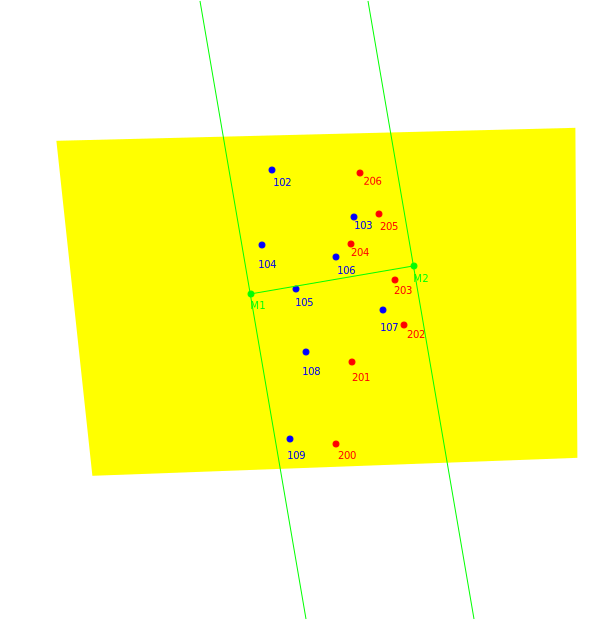
\includegraphics[scale=0.6]{RectDist.eps}
	\caption[Punkte mit einem rechtwinkeligen Abstand zur Schwerpunktlinie]{Alle Punkte von $B_1$ und $B_2$, die in dem Streifen zwischen den beiden Schwerpunkten liegen.}
	\label{fig:RectDist}		
\end{figure}


Nun nimmt man aus jeder Liste die beiden oberen Punkte und betrachtet sich die Linie, die sich zwischen diesen Punkten aufspannt. Schneidet diese Linie keines der beiden Polygone (außer an den Endpunkten), so merkt man sich den Mittelpunkt der Linie in der Liste: $Mittelpunktlinie$. Aus den Listen wird nun der größere der beiden Punkte gelöscht, falls dieser nicht der letzte in der Punktliste ist. Dieses Vorgehen wird solage vortgesetzt, bis beide Listen nur noch ein einziges Element haben. Die fiktiven Verbindungslinien und ihre Mittelpunkte sind auf der Abbildung~\ref{fig:Mittelpunkte} zu sehen.

\begin{figure}
	\centering
	\includegraphics[scale=0.6]{Mittelpunkte.eps}
	\caption[Verbindungslinien und deren Mittelpunkte]{Alle gefilterten Punkte aus $B_1$ und $B_2$, die zulässigen Vergindungslinien und deren Mittelpunkte.}
	\label{fig:Mittelpunkte}
\end{figure}

Der Linienzug, der nun in der Liste $Mittelpunktlinie$ liegt, liegt genau zwischen den beiden Polygonen und bildet die Struktur der Polygone an der Stelle ab, wo die beiden Polygone einander zugewant sind. Dieser Linienzug ist unter Abbildung~\ref{fig:MittelpunktLinie} zu sehen.

\begin{figure}
	\centering
	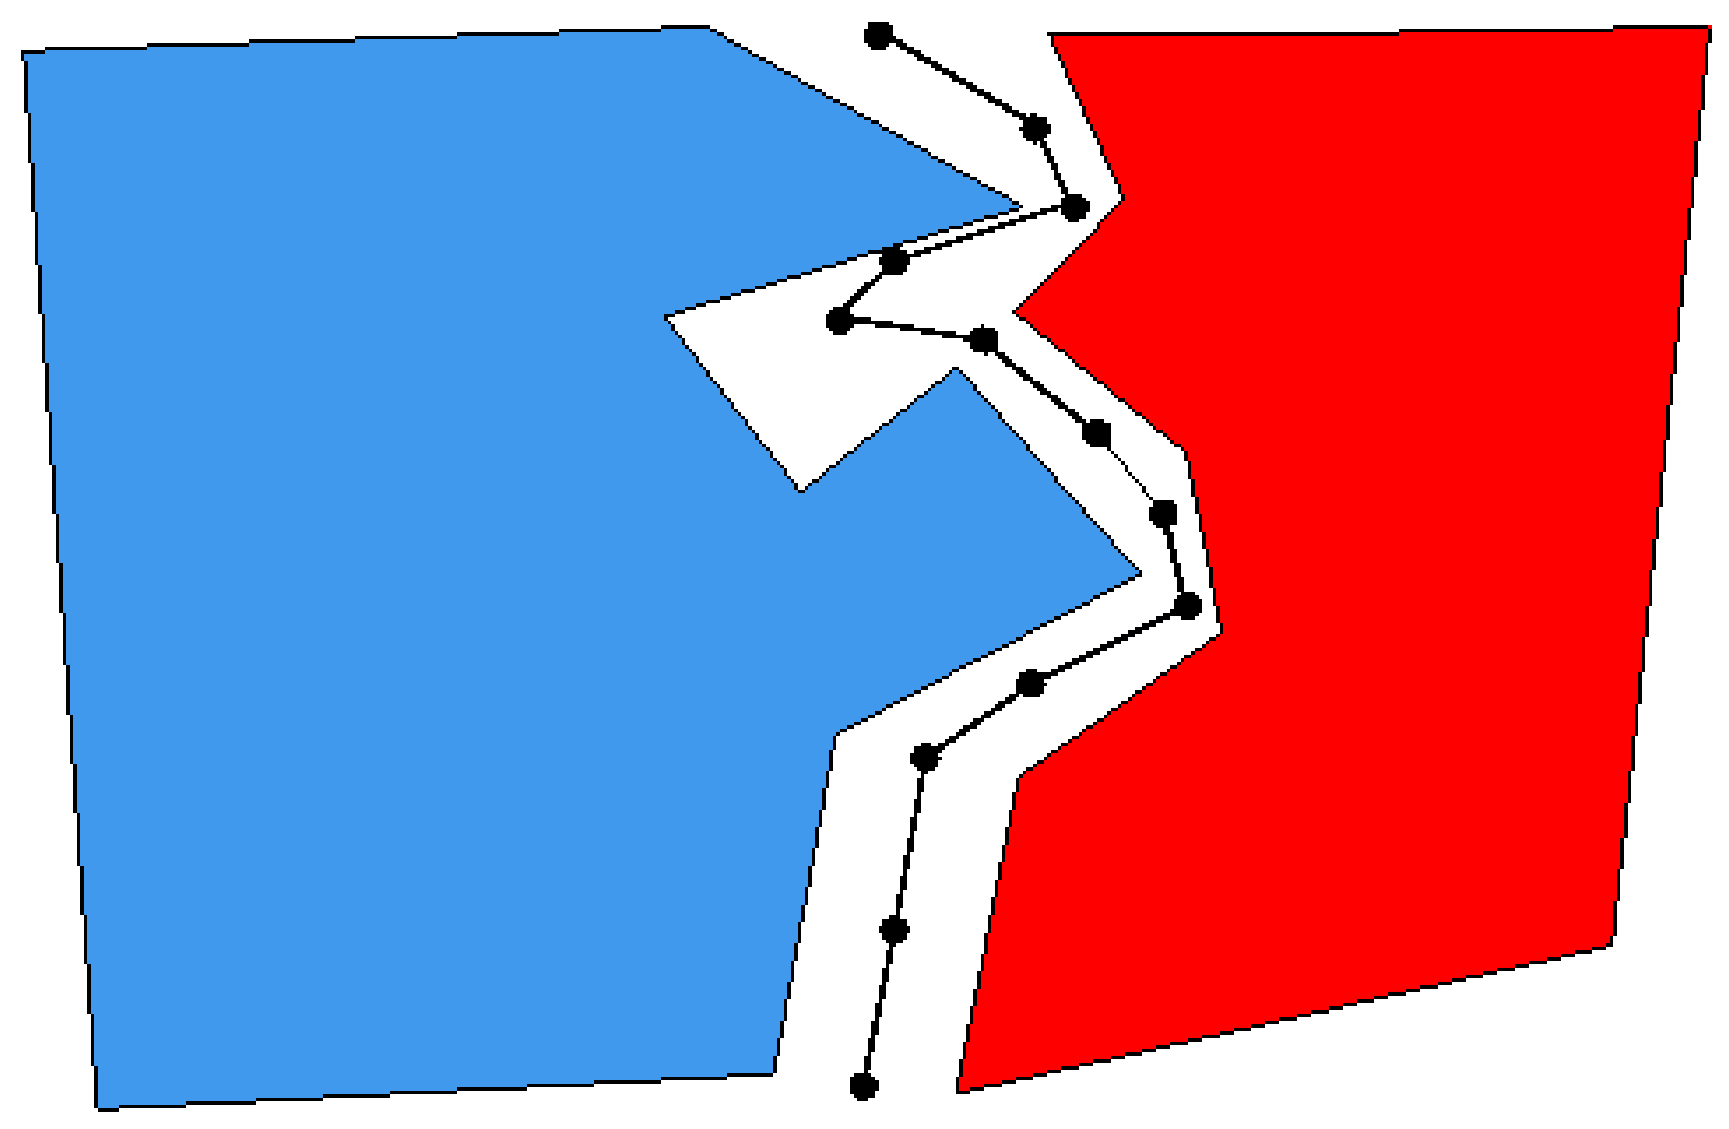
\includegraphics[scale=0.6]{MittelpunktLinie.eps}
	\caption{$B_1$ und $B_2$ mit dem berechneten Linienzug.}
	\label{fig:MittelpunktLinie}
\end{figure}

In der Regel teilt diese Linie  nun aber $A$ nicht, wie man an dem Beispiel gut sehen kann. Damit diese Linie nun wirklich duch $A$ geht, $A$ komplett geteilt wird und die Lage von $B_1$ und $B_2$ trotzdem noch wiedergespiegelt werden, führe ich folgende Schritte aus:

\begin{enumerate}
\item Berechne die Schwerpunkte $M_L$ der Linieneckpunkte, $M_A$ von $A$ und $M_B$ aller Eckpunkte von $B_1$ und $B_2$.
\item Berechne den Skallierungsfaktor $s_1=\frac{|A|}{|B_1|+|B_2|}$. 
\item Berechne das Maximum der Entfernungen von $M_L$ zu den beiden Endpunkten des Linienzuges, $d_L$ 
\item Berechne die maximale Entfernung von $M_A$ zu den Eckpunkten von $A$, $d_A$.
\item Berechne den Skallierungsfaktor $s_2=\frac{d_A}{d_l} * 1,05$. Die 5\% sind wilkürlich gewählt, und sollen die Warscheinlichkeit erhöhen, dass beide Endpunkte des neuen Linienzuges außerhalb von $A$ liegen. 5\% haben sich duchaus bewährt.
\item Berechne den neuen Linienzug $l'_1,l'_2,\hdots ,l'_n$ durch $l'_i=M_A+(l_i-M_l)*s_1+(M_l-M_B)*s_2$.
\end{enumerate}


Abbildung~\ref{fig:SplitLine} zeigt das Ergebniss an unserem Beispiel. 

Wie man schon an dem wilkürlichen Faktor 5\% sehen kann, liefert dieser Algorithmus bestimmt nicht in allen Fällen ein zulässiges Ergebnis. Die Erfolgsquote scheint aber sehr hoch zu liegen, in allen Beispielen, die ich beim Entwickeln durchgespielt habe tauchte kein einziger Fall auf, wo der Splitt versagte. Die Ergebnisse sahen auch alle sehr natürlich aus.


\begin{figure}
	\centering
	\includegraphics[scale=0.6]{Ergebnis.eps}
	\caption{Das Polygon $A$ mit der berechneten SplitLine.}
	\label{fig:SplitLine}
\end{figure}


\subsubsection{Zerteilete Löcher als Konkativitäten in ein Cycle einbauen}\label{JoinLL}

Wenn es bei der Teilung eines Faces dazu kommt, dass auch ein Hole geteilt wird, so werden aus den beiden neuen Polygonen Konkavitäten in den beiden neuen Faces. Zunächst muss jede dieser Konkativitäten dem passenden Face zugeordnet werden. Hierzu sucht man sich einfach einen Punkt des neuen Polygons der nicht auf dem Rand eines Faces liegt. Das passende Face ist dann dasjenige, in welchem der gewählte Punkt liegt. 

Als Beispiel betrachen wir das Polygon $A$ aus dem letzten Abschnitt als Face und ergänzen dieses durch ein Hole. Als Schnittlinie wird die eben berechnete benutzt. (siehe Abbildung~\ref{fig:JLL1})

\begin{figure}
	\centering
	\includegraphics[scale=0.6]{JLL1.svg.eps}
	\caption[EinFace mit einem Hole wird geteilt]{$A$ aus dem letzten Beispiel, jetzt um ein zu teilendes Hole ergäntzt.}
	\label{fig:JLL1}
\end{figure}

Der Algorithmus zum Vereinigen der Polygone bekommt nun also zwei Polygone, als geordnete Listen von Eckpunkten, das neue Face und ein passendes Bruckstück eines Holes. Diese Punktlisten werden zunächst sortiert. Die Punkte des Face werden wie gewöhnlich gegen den Uhrzeigersinn  angeordnet, die des Holes hingegen im Uhrzeigersinn. Zunächst suchen wir einen Punkt auf dem Rand des Faces, der nicht auf dem gemeinsamen Rand von Hole und Face liegt. Im Beispiel wählen wir Punkt 0.

Jetzt gehen wir die Punkte des Faces durch, solange auf der Linie zwischen dem aktuellen Punkt und dem Nächsten kein Punkt des Holes liegt. Alldiese Punkte fügen wir der Ergebnissliste $res$ hinzu.

Also: $rs=(0, 1, 2, 3, 4, 5)$.

Dann suchen wir aus allen Punkten des Holes, die auf der Linie von 5 zu 6 liegen, den Punkt der am nächstn zu 5 liegt. In unserem Fall ist das 107, den wir wieder an $res$ anhängen. Dieses etwas kompliziert klingende Vorgehen deckt eine Reihe von Sonderfällen ab, die hier auftauchen können. Abbildung~\ref{fig:SonderfaelleJLL} zeigt diese exemplarisch.

$res=(0, 1, 2, 3, 4, 5, 107)$

Nun durchlaufen wir die Punkte des Holes, beginnend mit 100, solange, bis der aktuelle Punkt auf dem Rand des Faces liegt (hier 103). Alle besuchten Punkte werden an $res$ angehängt.

Daraus folgt: $res=(0, 1, 2, 3, 4, 5, 107, 100, 101, 102, 103)$

Anschließend durchlaufen wir wieder das Face, wobei wir bei 6 beginnen, und suchen den ersten Punkt, der nicht auf dem Hole liegt. Im Beispiel ist dies Punkt 9.

Abschließend hängen wir an $res$ alle Punkte an, bis wir wieder am Ausgangspunkt angelangt sind.

Schließlich ist $res=(0, 1, 2, 3, 4, 5, 107, 100, 101, 102, 103, 9, 10, 11, 12)$. Abbildung~\ref{fig:JLL3} zeigt das Ergebniss als Polygon.


\begin{figure}
	\centering
	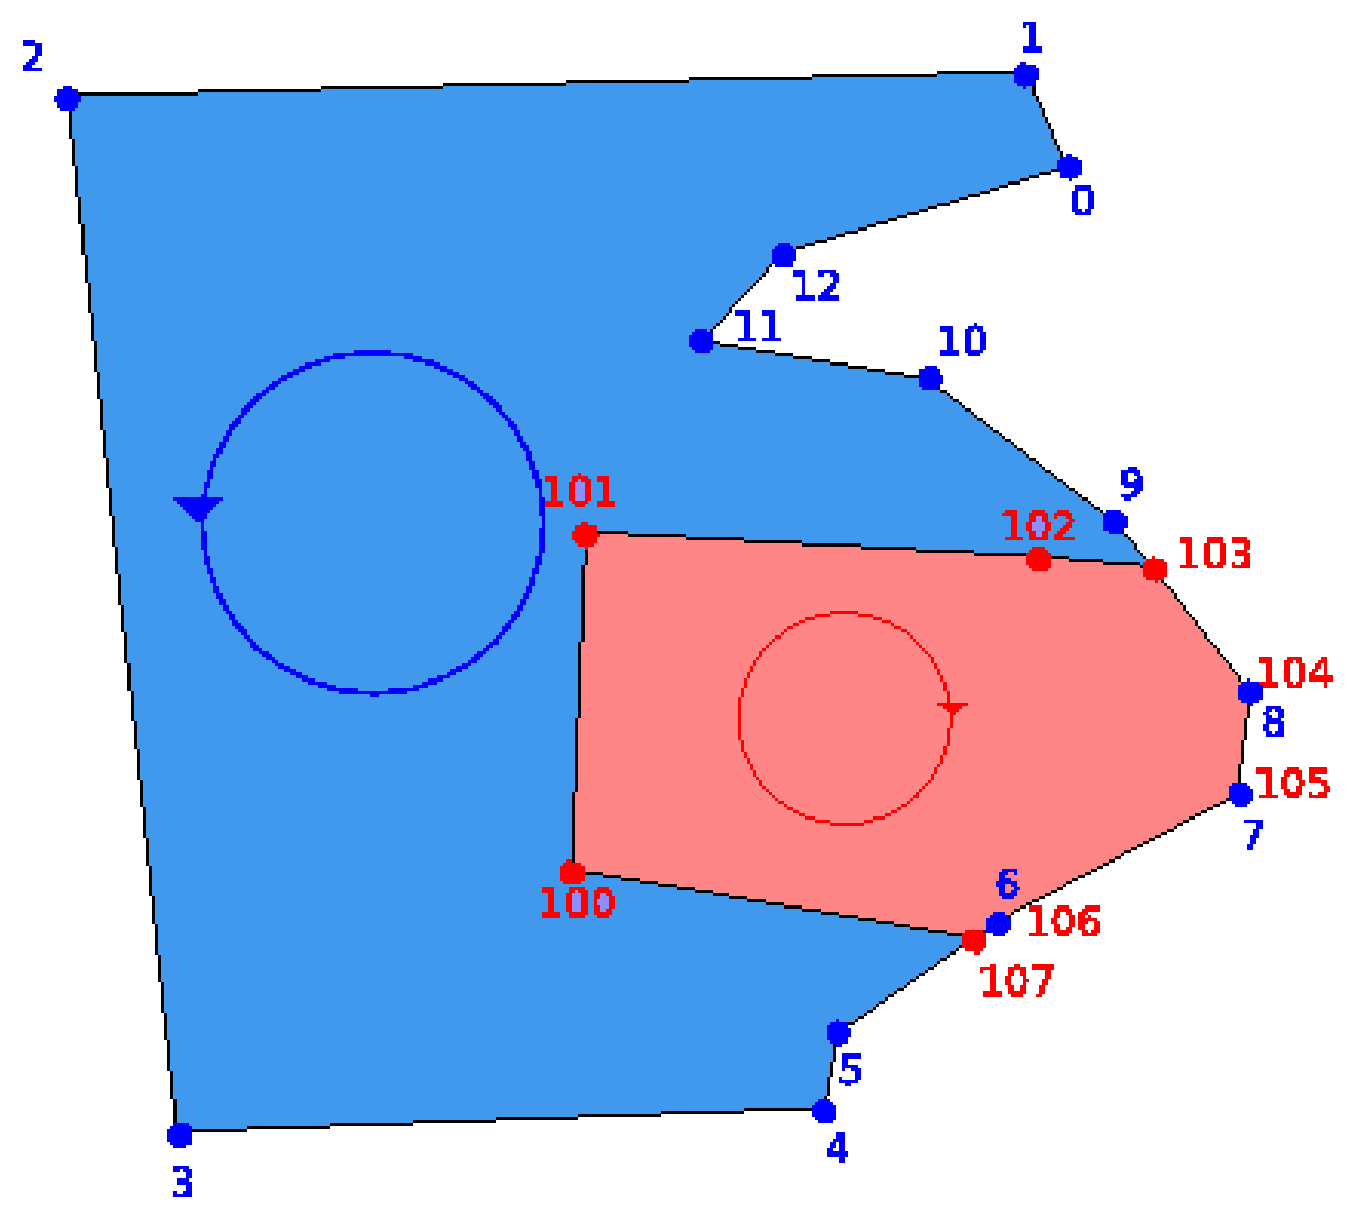
\includegraphics[scale=0.6]{JLL2.svg.eps}
	\caption{Die beiden neuentstandenen Polygone sollen verbunden werden.}
	\label{fig:JLL2}
\end{figure}


\begin{figure}
\subfigure[Beide Berührungspunkte liegen auf der selben Facelinie.]{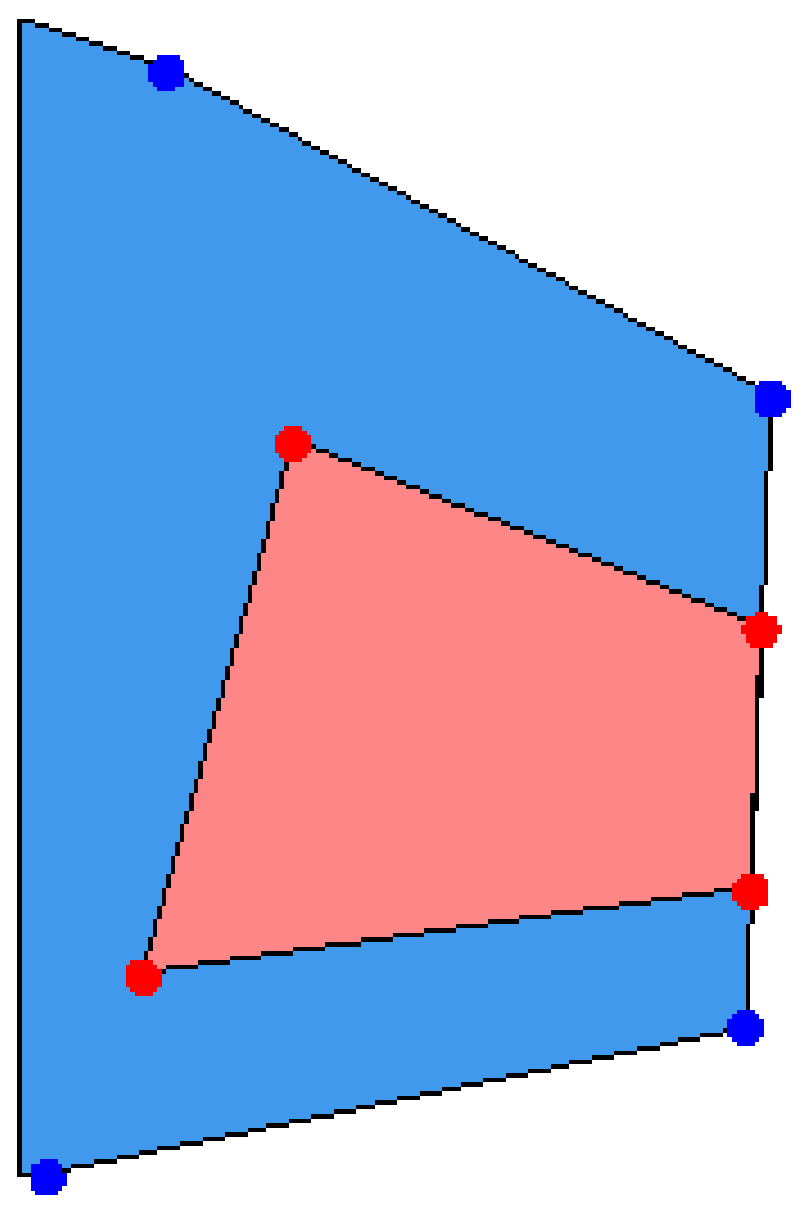
\includegraphics[width=0.35\textwidth]{Sonderfall1JLL.svg.eps}}\hfill
\subfigure[Der erste Punkt des Holes ist auch ein Punkt des Faces]{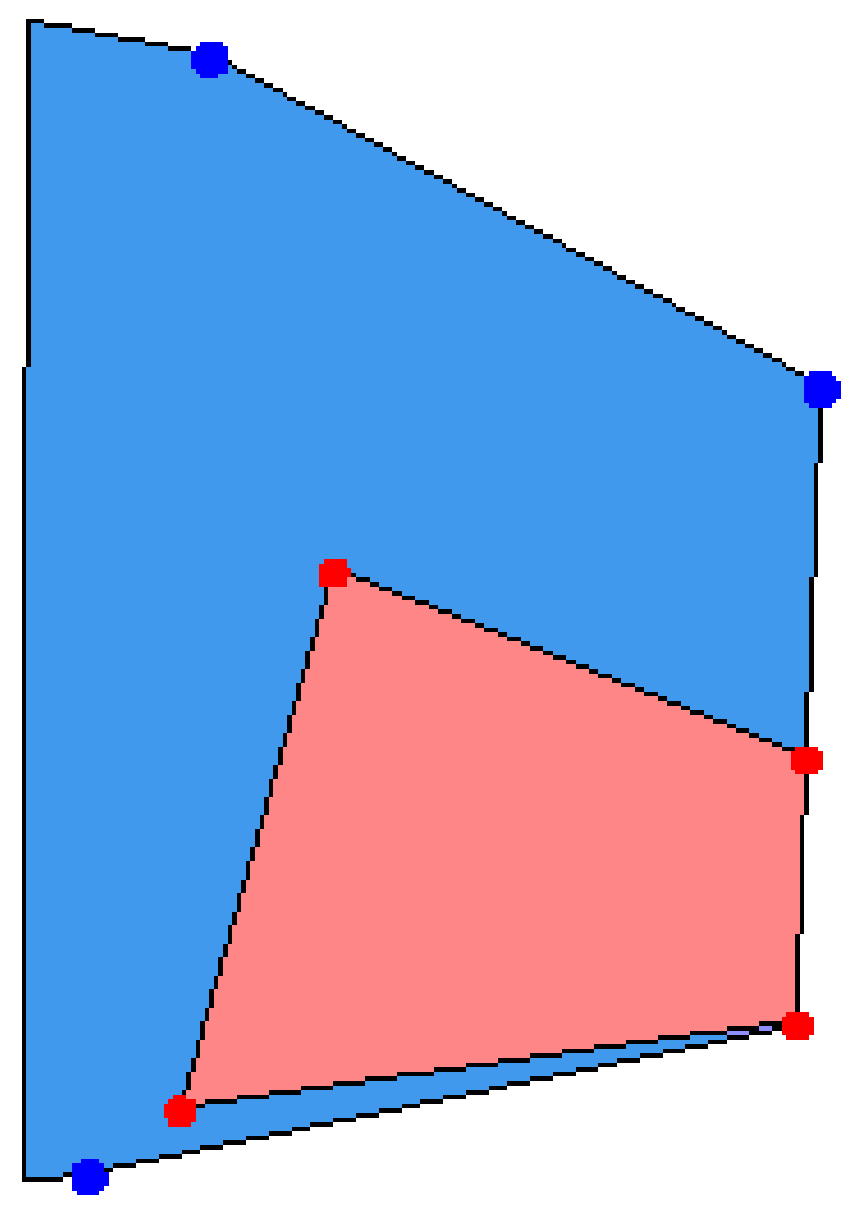
\includegraphics[width=0.35\textwidth]{Sonderfall2JLL.svg.eps}}
\caption[Sonderfälle, die bei der Vereinigung auftreten können]{Sonderfälle, die bei der Vereinigung auftreten können und wegen denen man die Funktion $getClosestBoundaryPoint$ benötigt.}
\label{fig:SonderfaelleJLL}
\end{figure}



\begin{figure}
	\centering
	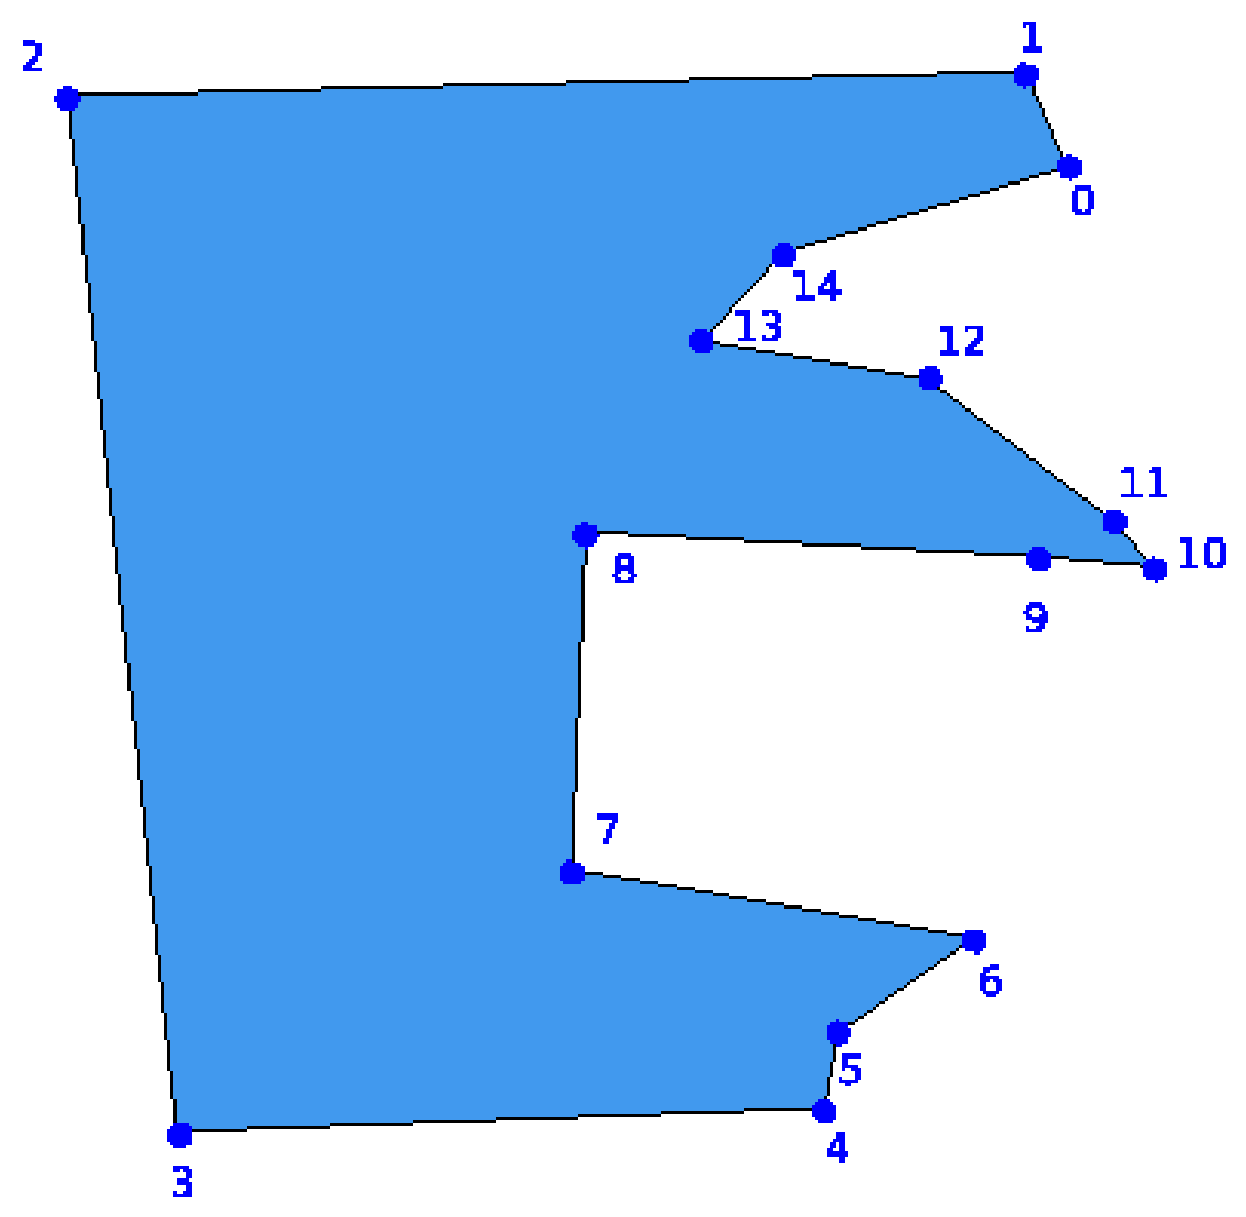
\includegraphics[scale=0.6]{JLL3.svg.eps}
	\caption{Das fertig zusammengesetzte Polygon.}
	\label{fig:JLL3}
\end{figure}



\subsubsection{\index{Rotaring Pane}Rotaring Pane} \label{rotPane}
In \cite{TG} wurde bereits der Algorithmus ,,rotating Pane'' vorgestellt. I, Laufe meiner Arbeit musste ich diesen Algorithmus nachprogrammieren, und habe hierbei eine Version gefunden, die etwas einfacher ist und erheblich weniger Fallunterscheidungen benutzen muss.

Die Idee dieses Algorithmusses ist es zu jeder Kante den Winkel zu bestimmen, den dieser mit der x"~Achse einnimmt. Zu zwei Ecken, die eine gemeinsame Kante bilden konstruiert man ein Dreieck mit dem Startpunkt der Kante des anderen Polygones zu bilden, dessen Winkel zwischen den Winkeln des Startpolygones liegt.

\begin{figure}
	\centering
	
\includegraphics{feu_logo2.eps}
	\caption[Tabellendarstellung des ,,rotating Pane'']{Diese Abbildung zeigt die beiden Felder zweier Vierecke und zeigt, welche Punkte zusammen ein movingsegment bilden.}
	\label{fig:RotatinPane}
\end{figure}


Hierzu werden zwei Felder von Punkten gebildet, für jeder Polygon eines. Zu Punkt jedem Punkt wird dann der Winkel hinzugefügt, den die Linie hat, welche von diesem Punkt ausgeht. Die Felder werden dann nach diesen Winkel sortiert. Zu zwei aufeinanderfolgenden Punkten der ersten Polygones wird dann der passende Punkt aus dem anderen Polygon gesucht. Hierzu wird die Funktion ,,finde\_passenden\_Index'' benutzt, die weiter unten erklärt wird. Das so entstandene Dreieck (als movingsegment) wird dann der Rückgabestruktur hinzugefügt.

\begin{algorithm}[!ht]
		\SetKwFunction{fMI}{finde\_passenden\_Index}
	\caption{Rotaring Pane Allgorithmus, um aus zwei konvexen H"ullen moving segments zu erstellen}
	\Ein{KH"ulle1 und KH"ulle2, zwei konvexe H"ullenb"aume}
	\Ergebnis{Eine Menge von moving segments, die die Interpolation der beiden Polygone darstellt}
	\Begin{
		Bestimme $KH1$ und $KH2$ die konvexen H"ullen der Polygone als Feld von LineWAs\;
		Berechne die Winkel in jedem Eckpunkt von $KH1$ und $KH2$\;
		Sortiere $KH1$ und $KH2$ aufsteigend nach diesen Winkeln\;
		$j:=0$\;
		\Fuer{$i<KH1.l"ange$}{
			$j:=\fMI{KH2, j, KH1[i].winkel, \text{false}}$\;
			F"uge das moving segment:$(KH1[i],KH1[i+1],KH2[j]$ dem Ergebnis-Feld hinzu\;
}			
		$j:=0$\;
		\Fuer{$i<KH2.l"ange$}{
			$j:=\fMI{KH1, j, KH2[i].winkel,\text{true}}$\;
			F"uge das moving segment:$(KH2[i],KH2[i+1],KH[j]$ dem Ergebnis-Feld hinzu\;
}			
}
\end{algorithm}


Diese Funktion durchsucht ein Feld, dass ein konvexes Polygon in der Form wie oben darstellt, nach dem übergebenen Winkel. Die Suche startet bei dem Index ,,Startindex''. Je nach dem Wert des Winkels an der angegebenen Stelle wird nach linkls oder rechts rekursiv weitergeangen. Sollten zwei Winkel exakt gleich sein, die Kanten also parallel sein, so muss man das Ergebniss unterschiedlich behandeln. Dieses leistet der Wert ,,Gleiche\_Winkel''.

\begin{function}[!ht]
	\caption{finde\_passenden\_Index(Polygon, Startindex, Winkel, Gleiche\_Winkel)}
	
	\Ein{\begin{tabular}{ll}
		Polygon: &Das zu durchsuchende konvexe Polygon als Feld\\
 			&von LineWAs\\
		Startindex: &Der Index, an dem die Suche beginnen\\
 				&soll\\
		Winkel: &Der Winkel, zu dem der passende Index gesucht\\
 			&wird\\
		Gleiche\_Winkel: &Dieser boolsche Parameter gibt an, \\
				&wie mit parallelen Kanten verfahren werden soll
	     \end{tabular}
}
	\BlankLine
	\Ergebnis{Der Index des Punktes, an dem die Linie anf"angt, mit der die Ecke mit dem "ubergebenen Winkel gematched wird}
	\Begin{	
        	\uWenn {$Winkel<Polygon[0].Winkel$}	{
        		Gebe den Index 0 zur"uck\;
}
        	\uWenn{$Polygon[0].Winkel=Winkel$ und $Gleiche\_Winkel$}{
        			Gebe den Index 0 zur"uck\;
}        
        	\Wenn{$Winkel>Polygon[letzer\_Index].Winkel$}{
        		Gebe den Index 0 zur"uck\;
}
	
        	\Solange{Nicht $(Polygon[j].Winkel\geq Winkel$ und $Polygon[j-1].Winkel\leq Winkel)$}{
        		\uWenn{$(j\neq0$ und $Winkel<Polygon[j-1].Winkel$}{
        			$j:=j-1$\;
}	
 	           	\Sonst{
				\Wenn{$Polygon[0].Winkel\neq Winkel$}{
		                 	$j:=j+1$\;
}
}
}
		\Wenn{$Polygon[j].Winkel=Winkel$ und $Gleiche\_Winkel$}{
	        	$j:=j+1$\;
}
		Gebe den Index $j$ zur"uck\;
}		
\end{function}

\clearpage

\subsubsection{Zerlegung von einfachen Polygonen in konvexe Polygone}\label{Zerlegung}

Um beliebige Polygone in VRML-Dateien exportieren zu können, musste ich einen Algorithmus finden, der beliebige, einfache Polygone in konvexe zerlegen kann. Natürlich hätte ich einfach eine Dreieckszerlegung vornehmen können, diese Zerlegung wäre aber möglicherweise erheblich kleinteiliger, als ich das eigentlich brauchte. Die Idee des Algorithmusses ist auch ganz einfach:

Ecken, deren Wickel größer als 180\degree\/ sind, so genannte konvexe Ecken, stören und müssen beseitigt werden. Teile ich ein Polygon an einem Winkel, so wird dieser kleiner. Also kann man Polygon solage, an konvexen Ecken,  zerteilen, bis es in keinem der Ergebnisspolygone noch einen konvexen Winkel gibt.

Teilen kann man ein Polygon an zwei Ecken $A$ und $B$, falls die Verbindung von $A$ und $B$ innerhalb des Polygones liegt, und keine unbeteiligte Kante geschnitten wird.

Verbessen kann man diesen Ansatz noch dardurch, dass man zuerst versucht das Polygon an zwei konvexen Ecken zu teilen.

Dieser Algorithmus funktioniert nicht nur für einfache Polygone, sondern auch für solche, in denen eine Kante zweifach durchlaufen wird. Damit kann man auch Faces mit Holes zerlegen.

\begin{figure}
	\centering
	
\includegraphics{feu_logo2.eps}
	\caption{Ein Beispiel, wie ein Face mit einem Hole in konvexe Polygone zerfällt.}
	\label{fig:ZerlegungFace}
\end{figure}


\begin{algorithm} [!ht]
	\SetKwFunction{gCV}{liefere\_konvexe\_Ecken}
	\SetKwFunction{iSA}{ist\_teilbar}
	\caption{Zerlegung von einfachen Polygonen in konvexe Polygone}
	\Ein{Eine Menge $Polygone$ von einfachen Polygonen, repr"asentiert durch geordnete Punktlisten}
	\Ergebnis{Die Menge $Polygone$ besteht nur noch aus konvexen Polygonen}
	\Begin{
		$aktuell:=0$\;
		$konvexe\_Ecken=\emptyset$\;
		\Wiederh{$|konvexe\_Ecken|=0$ und $aktuell=|Polygone|$}{
            		$aktuelles\_Polygon=Polygone[aktuell]$\;
			$konvexe\_Ecken=aktuelles\_Polygon.\gCV{}$\;
			\uWenn{$|konvexe\_Ecken|>0$}{
				\Wenn{$|konvexe\_Ecken|>1$}{
					\Fuer{$i<|konvexe\_Ecken|$}{
						\Fuer{$j:=i+1$ \KwTo $j<|konvexe\_Ecken|$}{
							\Wenn{$aktuelles\_Polygon.\iSA{konv\_Eck[i],konv\_Eck[j]}$}{
								Teile $aktuelles\_Polygon$ an den Ecken $konvexe\_Ecken[i]$ und $konvexe\_Ecken[j]$\;
								Ersetzt $aktuelles\_Polygon$ in $Polygone$ durch die beiden neuen Polygone\;
								Durchlaufe alle Scheifen von neuem\;
}
}
}
}
                		$Index1:=konvexe\_Ecken[0]$\;
				$Index2:=Index1+\frac{|aktuelles\_Polygon|}{2}$\;
				\Fuer{$i<|aktuelles\_Polygon|$}{
					$split\_Index=Index2+\frac{(-1)^i i}{2}$\;
		                    	\Wenn{$aktuelles\_Polygon.\iSA{Index1,split\_Index}$}{
		                    	Teile $aktuelles\_Polygon$ an den Ecken $Index1$ und $split\_Index$\;
								Ersetzt $aktuelles\_Polygon$ in $Polygone$ durch die beiden neuen Polygone\;
}
}
}
			\Sonst{
				$aktuell:=aktuell+1$\;
}

}
}
\end{algorithm}

\clearpage

\subsubsection{\index{ConvexHullTreeNode!Konstruktion}Aufbau eines ConvexHullTrees}\label{constCHTN}
Der Algorithmus zum Aufbau eines ConvexHullTrees wurde in \cite{TG} bereits erl"autert. Da dieser aber von zentraler Bedeutung zur L"osung des Problems ist, bespreche ich den Algorithmus an dieser Stelle noch einmal.

Als Beispiel dient mir ein Polygon aus der GERMANY-Datenbank. Bei diesem Polygon handelt es sich um die Gemeinde Sandershausen, die als Enklave zu dem Stadtkreis Kassel geh"ort. Abbildung~\ref{fig:Sanders} zeigt dieses Polygon in dem dazugeh"origen Luftbild, dass ich aus der Applikation Google-Earth entnommen habe. 

Der erste Schritt, bei der Erzeugung eines ConvexHullTree-Kontens, ist die Ereugung der konvexen H"ulle des Polygons. In den Abbildungen~\ref{fig:sand2} ist diese in Rotbraun eingezeichnet. Der Allgorithmus, der zur Erzeugung der H"ulle benutzt wird ist der \index{Graham Scan}Graham Scan Algorithmus, der zu den Standard-Allgorithem zu z"ahlen ist. In \cite{G72} wurde dieser Algorithmus das erste Mal beschrieben. Eine gute Beschreibung finden Sie \anmerkung{hier Literaturstelle einf"ugen}.

Im Anschu"s daran wird das Ausgangspolygon nach zusammenh"angenden Linienz"ugen durchsucht, die nicht in der konvexen H"ulle enthalten sind. Diese Suche wird mittels eines parallelen Durchlaufs duch beide Linienz"uge realisiert.

Schlie"slich wird diser Algorithmus rekursiv f"ur alle diese Linienz"uge aufgerufen und die Ergebnisse werden an die entsprechenden Stellen in den Vaterknoten eingeh"angt.

\begin{figure}
	\centering
	\includegraphics[width=10cm]{Sandershausen.eps}
	\caption{Die Gemeinde Sandershausen als Beispiel eines ConvexHullTrees}
	\label{fig:Sanders}
\end{figure}
\begin{figure}
\subfigure[die Nodes der Level 0-1]{\includegraphics[width=0.45\textwidth]{Sandershausen2.eps}}\hfill
\subfigure[kompletter ConvexHullTree]{\includegraphics[width=0.45\textwidth]{Sandershausen3.eps}}
\caption{Ausschnitt von Sandershausen mit verschieden detailierten ConvexHullTrees}
\label{fig:sand2}
\end{figure}
%\begin{figure}%
	%\centering
	%\includegraphics[width=5cm]{Sandershausen2.eps}
	%\caption{Ausschnitt von Sandershausen mit den Nodes der Level 0-1}
	%\label{fig:sand2}
%\end{figure}
%\begin{figure}
%	\centering%
	%\includegraphics[width=5cm]{Sandershausen3.eps}
	%\caption{Ausschnitt von Sandershausen mit dem kompletten ConvexHullTree}
	%\label{fig:sanders3}
%\end{figure}

\begin{algorithm}[!ht]

\SetKwFunction{cH}{berechne\_konvexe\_H"ulle}
	\caption{Erzeuge einen konvexen H"ullenbaum aus einem Polygon}
	\Ein{\begin{tabular}{ll}
		Polygon: &Ein Polygon,rep"asentiert duch eine geordnete Liste von \\
			&Eckpunkten\\
		Ebene:	&Die Ebene des zu Erzeugenden Elementes\\
		ist\_Loch: &Ein boolscher Parameter der angibt, ob das neue Element \\
			&zu einem Loch geh"ort\\
		Vater:	&Das Vaterelement des Neuen\\
		\end{tabular}
}
	\BlankLine
	\Ergebnis{Ein konvexer H"ullenbaum, der das "ubergebene Poygon beschreibt}
	\Begin{
	
%         LineWA[] tmplist, convhull, childlist;
	Setze die Klassen-Variabeleln $ist\_Loch$ und $Vater$\;

%         int node;
%         int index1, index2, length, lastindex, noiterations;
%         int indexll1, indexll2;
%         this.linelist = new Vector();
%         smallesty = Integer.MAX_VALUE;
%         smallestx = Integer.MAX_VALUE;
%         smallestpoint = -1;       
	$konvexeH"ulle:=\cH(Polygon)$\;
%         // Find where the first node in linelist is in the convex hull
%         // (Or the earliest possible if the first node is not on the hull)
%         // This is to preserve the order in the linelist in the ordering of
%         // points in the convex hull tree node.
	$startindex:=0$\;
	$endindex:=konvexeH"ulle.L"ange$\;
	Finde den Index, in der konvexen H"ulle, der dem niedrigsten Index in dem Polygon entspricht, und speichere Ihn in $startindex$\;
	Finde den Index, in der konvexen H"ulle, der dem h"ochsten Index in dem Polygon entspricht, und speichere Ihn in $endindex$\;
         %for (int a=0;a<linelist.length;a++)
% {
%             index1 = TriRepUtil.indexOf(convhull, linelist[a]);
%             if (index1 != -1) break;
% }
%         for (int a=linelist.length-1;a>=0;a--)
% {
%             lastindex = TriRepUtil.indexOf(convhull, linelist[a]);
%             if (lastindex != -1) break;
% }
	\uWenn{$startindex<endindex$}{
		\Fuer{$i:=startindex$ \KwTo $i\leq endindex$}{	
			Speichere $konvexeH"ulle[i]$ in der linelist des neuen Konten\;
}
}
	\Sonst{
		
        	\Fuer{$i:=index1$ \KwTo $konvexeH"ulle.L"ange$}
{
			Speichere $konvexeH"ulle[i]$ in der linelist des neuen Konten\;
}
		\Fuer{$i:=0$ \KwTo $endindex$}
{
			Speichere $konvexeH"ulle[i]$ in der linelist des neuen Konten\;
}
}
%         // Check lines in convex hull with lines in line list. Whenever two points
%         // which are neighbours in the convex hull are not neighbours in the line
%         // list, create a child node from the points between them.
%         
%         noiterations = numberOfLines();
%         index1 = 0;
%         indexll1 = 0;
%         while (!(linelist[indexll1].equals(getLine(index1))))
% {
%             indexll1++;
% }
	\Fuer{$i<konvexeH"ulle.L"ange$}
{
%             index2 = index1+1;
%             indexll2 = indexll1+1;
%             while (!(linelist[indexll2 % linelist.length].equals(getLine(index2 % noiterations))))
% {
%                 indexll2++;
% }
%             
%             if ((indexll2 != indexll1+1) && ((level == 0) ||
%                     ((indexll2 != linelist.length) && (indexll1 != linelist.length-1)))
%                     && (indexll2 != indexll1-1))
% {
%                 // create child node
%                 length = indexll2-indexll1+1;
%                 childlist = new LineWA[length];
%                 for (int b=0;b<length;b++)
% {
%                     if ((b+indexll1) < linelist.length)
% {
%                         childlist[length-b-1] = linelist[b+indexll1];
% }
%                     else
% {
%                         childlist[length-b-1] = linelist[b+indexll1-linelist.length];
% }
% }
%                 insertChild(index1, new ConvexHullTreeNode(childlist, level+1,this.isHole,this));
% }
%             index1 = index2;
%             indexll1 = indexll2;
}
}
 \end{algorithm}

\clearpage
\subsubsection{Bestimmung der maximalen Distanz mehrerer Polygone}\label{maxDist}
\label{gmD}
Die Berechnung der größten Abstandes den zwei Punkte aus verschiedenen Polygonen ist eine relativ aufwendige Operation, mit quadratischem Aufwand. Dieser Algorithmus liefert einen sehr ähnlichen Wert in $O(n\log(n))$. Dieser Wert ist der Durchmesser der konvexen Hülle der Punkte beider Polygone. 

Zur Berechnung dieses Wertes wird zuerst die gemeinsame konvexe Hülle der beiden Polygone berechnet. Dann wird von jedem Punkt der konvexen Hülle die maximale quadratische Distanz berechnet und die Wurzel der größten Distanz zurückgegeben.

\begin{algorithm}[!ht]
	\SetKwFunction{gLDFP}{l"angste\_Entfernung\_von\_Punkt}
	\SetKwFunction{dist}{Quadrat\_der\_Entfernung}
	\caption{Bestimmung der maximalen Distanz mehrerer Polygone}
	\Ein{Mehrere Polygone repr"asentiert duch ihre Punktlisten}
	\Aus{Der maximale Abstand von zwei Punkten}
	\Begin{
		Bilde eine gemeinsame Punktliste durch konkatenieren der Eingangslisten\;
		Bilde $CH$ die konvexe H"ulle der Eingangsdaten\;
		$i:=0$\; 
		$tmpdist:=0$\;
		$pos:=\frac{CH.length}{2}$\;
		\Fuer{$i<CH.length$}{
			$pos:=\gLDFP{CH[i],CH,pos}$\;
			$distxy:=\dist{CH[i],CH[pos]}$\;
		        \Wenn{$distxy>tmpdist$}
{			
			           $tmpdist:=distxy$\;
}			
}    
		Das Ergebnis ist $\sqrt{tmpdist}$\;
}
\end{algorithm}
\clearpage

Diese Funktion sucht in einem konvexen Polygon den Punkt, der am weitesten von dem übergebenen Punkt entfernt ist. Der Punkt an dem Index Startindex ist der Punkt, mit dem zuerst verglichen wird. Die Suche läuft danach rekursiv weiter. 

\begin{function}[!ht]
	\SetKwFunction{dist}{Quadrat\_der\_Entfernung}
	\SetKwFunction{gLDFP}{l"angste\_Entfernung\_von\_Punkt}
	\caption{l"angste\_Entfernung\_von\_Punkt(Punkt, Polygon, Startindex)}
	\Ein{\begin{tabular}{ll}
Punkt: &Der Punkt, zu dem der Abstand gemessen wird,\\
	     Polygon: &Das konvexe Polygon, in dem der am weitesten \\
			&entfernte Punkt gesucht wird\\
	
	     Startindex: &Der Index an dem die Suche begonnen wird\end{tabular}}
	\BlankLine
	\Ergebnis{Der Index des Polygonpunktes, der von dem Punkt den maximalen Abstand hat.}
	\Begin{
		$distpos:=\dist{Punkt,Polygon[pos]}$\;
		$distposlinks:=\dist{Punkt,Polygon[pos+1]}$\;
		$distposrechts:=\dist{Punkt,Polygon[pos-1]}$\;
		\uWenn{$distpos\geq distposlinks$ und $distpos\geq distposrechts$}{
			Gebe $pos$ als Ergebnis zur"uck\;
}
		\Sonst{
			\uWenn{$distposlinks>distpos$}{
				Gebe $\gLDFP{Punkt, Polygon, (pos+1)}$ zur"uck\;
}		
			\Sonst{Gebe $\gLDFP{Punkt, Polygon, (pos-1)}$ zur"uck\;}
}
}
\end{function}

\label{getdist}
Diese Funktion liefert den Wert der quadratischen Entfernung von zwei Punkten zurück. Die Berechnung erfolgt nummerisch stabiler als die einfache Formel $(x_2-x_1)^2+(y_2-y_1)^2$. Besonders im Umgang mit geografischen Koordinaten ist dies wichtig.

\begin{function}[!ht]
	\caption{Quadrat\_der\_Entfernung(Punkt1, Punkt2)}
	\Ein{Die beiden Punkte, deren Abstand berechnet werden soll}
	\Ergebnis{Das Quadrat des Abstandes der beiden Punkte}
	\Begin{
		Berechne $x_1^2$ $x_2^2$, $y_1^2$, $y_2^2$, $x_1x_2$ und $y_1y_2$ in doppelter Genauigkeit\;
		Gebe $x_1^2+x_2^2+y_1^2+y_2^2-2(x_1x_2+y_1y_2)$ in einfacher Genauigkeit zur"uck\;
}
\end{function}


\clearpage
\subsection{Beschreibung der Klassen}\label{klassen}

\subsubsection{\index{LineWA}LineWA}

Diese Klasse repräsentiert einen zweidimensionalen Punkt, der durch eine Winkelangabe ergäntzt ist. Somit kann man ein Polygon speichern indem man alle seine Punkte speichert, und zu jedem Punkt noch den Winkel, den die Kante, die von dem Punkt ausgeht, mit der x"~Achse hat. Die Klasse ist so implementiert, dass mehrere LineWAs automatisch aufsteigen nach ihren Winkeln sortiert werden können.

\subsubsection{\index{CHLine}CHLine}

Die CHLine ist eine LineWA in einem ConvexHullTreeNode. Zusätzlich zu den bekannten Attributen kann diese auch noch einen ConvexHullTreeNode als Kind enthalten. Diese Klasse trägt quasi die rekursive Struktur des ConvexHullTrees.

\subsubsection{\index{LineDist}LineDist}

Diese Klasse dient dazu, Kombinationen von Punkten und Entfernungen speichern zu können. Wie bei der LineWA ist die Sortierung nach Entfernung möglich.

\subsubsection{\index{PointWNL}PointWNL}

Diese Klasse dient dazu Punkte im dreidimensionalen darstellen zu können.

\subsubsection{\index{ConvexHullTreeNode}ConvexHullTreeNode}

Diese Klasse repräsentiert den ,,konvexen Hüllenbaum'', der bereits öfter erwähnt wurde. Der ConvexHullTreeNode enthält an Attributen:

\begin{itemize}
\item linelist

Die linelist ist ein Feld von CHLines, enthält also alle Punkte der konvexen Hülle und die dazugehörigen Kinder.

\item level

Hiermit kann man feststellen, in welcher Tiefe sich ein ConvexHullTreeNode in dem ConvexHullTree befindet.

\item hole

Dieses boolsche Attribut legt fest, ob das Objekt zu einem Cycle,oder zu einem hole gehört.

\item myParent

Dieses Attribut zeigt auf das Vaterelement des Objektes in dem RegionTree. Der Vater kann entweder ein face, oder ein anderer ConvexHullTreeNode sein.

\end{itemize}

Die wichtigsten, nicht trivialen Methoden dieser Klasse sind:

\begin{itemize}
\item Konstruktor

Der Konstruktor ist näher unter \ref{constCHTN} beschrieben.

\item getLines

diese Funktion liefert die Punkte des Polygons zurück, die dieser ConvexHullTree beschreibt.

\item getCenter

liefert den Schwerpunkt der konvexen Hülle.

\item getSteinerPoint

liefert den Steinerpunkt der konvexen Hülle.

\item getSplitLine

liefert einen Linienzug, an dem das Objekt geteilt werden kann. Die beiden übergebenen konvexen Hüllenbäume dienen hierbei als Anleitung. Der entsprechende Algorithmus findet sich unter \ref{ZerteilungsAlgo}

\item getSplitNodes

diese Funktion teilt das Objekt an dem übergebenen Linienzug und liefert ein zweidimensionales Feld von Punkten zurück, die die beiden neuen ConvexHullTreeNodes repräsentieren.  

\end{itemize}


\subsubsection{\index{Face}Face}

Ein Face besteht aus einem Cycle und mehreren, oder keinem Hole. Sowohl der Cycle, als auch die Holes sind durch ConvexHullTrees gegeben. Die Attribute des Faces sind:

\begin{itemize}
\item Cycle

ein ConvexHullTreeNode, der das begrenzende Polygon dieses Faces beschreibt.

\item Holes

ein Feld von ConvexHullTreeNodes, das die Holes des Faces beinhalten.

\item parent

ein Verweis auf die Region (bzw. RegionForInterpolation), zu der dieses Face gehört.

\end{itemize}

Die wichtigsten, nicht trivialen Methoden dieser Klasse sind:

\begin{itemize}

\item getHolesAndConcavities

diese Funktion liefert alle Konkativitäten des Cycles, und alle Holes des Faces. Diese Funktion wird beim Matchen benötigt, da die Holes, und die Konkativitäten des Cycles zueinander gematcht werden können.

\item splitOnLine

diese Funktion teilt das Face, entlang des übergebenen Linienzuges, in zwei neue Faces. Das eine neue Face wird zurückgegeben, das andere ersetzt das vorherige Face. Mißlingt die Teilung, so wird $null$ zurückgegeben, und das Face selbst bleibt unverändert.

\end{itemize}

\subsubsection{\index{Region}\index{RegionForInterpolation}Region oder RegionForInterpolation}

Eine Region enthält ein oder mehrere Faces. In Secondo war der Name ,,Region'' leider schon für die Region in der SpatialAlgebra vergeben. Desshalb musste ich die Klasse dort in RegionForInterpolation umbenennen.

An Attributen enthält eine Region im Wesentlichen nur ein Feld von Faces.

Die einzige Methode, die nicht nur der Verwaltung der Faces dient, und etwas interesannter ist, ist 
\begin{itemize}
\item splitOnLine

diese Funktion versucht alle Faces an dem übergebenen Linienzug zu teilen, und ergäntzt die Liste der Faces um eventuell auftauchende Neue. Die Funktion liefert ausserdem eine Liste aller neuhinzugefügten Faces als Rückgabe, so dass direkt erkennbar ist, inwieweit diese Operation die Region verändert hat.

\end{itemize}

\subsubsection{\index{RegionTreeNode}RegionTreeNode}

Dieses Interface dient dazu, Region, Faces und ConvexHullTreeNodes gleichbehandeln zu k"onnen. Implementiert sind nur hashCode und equals, zum Auffinden von SingleMatches in HashSets. Die Berechnung des Hashwertes wird von den Klassen so implementiert, wie unter \ref{berechenHashwerte} beschrieben. Abbildung~\ref{fig:RegionTreeNode} zeigt den Aufbau eines RegionTrees schematisch.




\subsubsection{\index{SingleMatch}SingleMatch}
Diese Klasse repr"asentiert eine einzelnes Teilmatch.  Es enth"alt eine Source-Kom"-ponente und ein Feld von Target-Komponenten. Alle Komponenten sind RegionTreeNodes.
Die wichtigsten Methoden sind:

\begin{itemize}
\item Der Konstruktor

Der Konstruktor legt ein SingleMatch zwischen den Komponenten Source und Target an. Es kann nur ein einziges Target "ubergeben werden, weitere m"ussen mit addTarget hinzugef"ugt werden.



\item addTarget

Diese Methode f"ugt eine weitere Target-Komponente hinzu.

\item getNrTargets

Diese Methode liefert die Anzahl der Targets.

\item getTargetAt

Diese Methode liefert das Target mit dem "ubergebenen Index zur"uck.

\item removeTargets

Diese Methode l"oscht alle Targets dieses SingleMatches.

\item hashCode

Liefert den Hashwert des Matches.

\item equals

"Uberpr"uft zwei Komponenten auf Gleichheit.

\end{itemize}

Die beiden letzten Methoden dienen dazu, SingleMatches in einem HashSet ablegen zu k"onnen, wobei nur die source-Komponente f"ur das Auffinden des Matches herangezogen wird.

\subsubsection{\index{Match!Klasse}Die abstrakte Klasse Match}
Diese abstakte Klasse stellt die wesentlichen Mechanismen zur Verf"ugung, um einfach Matches programmieren zu k"onnen. Es enth"alt die Eigenschaften:
\begin{itemize}
\item source

Die Region zum Eingangszeitpunkt.

\item target

Die Region zum Ausgangszeitpunkt.

\item maps

Ein Hashtable, in dem die einzelenen Teilmatches abgelegt werden. Der Schl"ussel, um auf die Elemente dieses Tables zugreifen zu k"onnen ist die Quell-Komponente vom Typ RegionTreeNode.

\item name

Der Name des Matches.

\item description

Eine Beschreibung, wie das Matching funktioniert.

\item einige Attribute, die der Berechnung der Bewertungen dienen.
\end{itemize} 

Diese Klasse verf"ugt "uber einige Methoden, die wichtigen davon  sind:

\begin{itemize}

\item Der Konstruktor

Setzt Name, Beschreibung, Source und Target auf die angegebenen Werte und initialisiert ein leeres Hashtable.

\item addMatch

Diese Methode f"ugt ein neues Match von Source nach Target ein. Sollte es noch kein Match von Source aus geben, so legt er ein neues Match an, und erweitert anderenfalls das Vorhandene.

\item getMatches

Diese Methode liefert ein Feld mit allen Targets, die von Source aus gematcht sind.

\item removeMatches

Diese Methode löscht den übergebenen RegionTreeNode aus der Match-Struktur. Hierbei wird nicht nur das Single-Match gelöscht, dass das übergebene Objekt als Source hat, sondern es werden auch alle Targets durchsucht.

\item getTargetChildren

Diese Methode liefert alle Kinder der Targets als Feld aus. Falls ein Target ein ConvexHullTreeNode ist, dann finden sich im R"uckgabefeld alle seine Kinder  wieder, falls Target ein Face ist, dann werden alle Holes und die Kinder des Cycles zur"uckgegeben. Diese Sonderbehandlung des Faces ist n"otig, da man ein Face mit seinem Cycle identifizieren kann, und die L"ocher also quasi Kinder des Cycles sind.

\item finalize

Die Erzeugung von Dreiecken bzw. MovingLines mit der Klasse mLineRep funktioniert nur, falls auschließlich 1:1 Matchings vorkommen. Nach der Erzeugung des Matchings ist das im Allgemeinen nicht gew"ahrleistet, deshalb muss man am Ende der Erzeugung diese Methode aufrufen, die sich darum k"ummert (siehe \ref{1zuN}). Auch die Beseitigung von zu stark gedrehten Konkativit"aten (siehe \ref{gedrehtKon}) findet hier statt.

\item Die Bewertungsfunktionen

In dieser Klasse sind auch einige der Bewertungsverfahren implementiert, die ich unter \ref{bewertung} beschrieben habe. Im einzelnen sind dass:
\begin{itemize}
\item Das Area-Rating
\item Das Hausdorff-Rating
\item Das Linear-Rating
\item Das Overlap-Rating
\end{itemize}

\item getRating

diese Funktion bekommt vier Gewichte, multipliziert jedes Rating mit seinem Gewicht, und liefert diese gewichtete Summe zurück.

\end{itemize}


Folgende abstrakte Methoden müssen von abgeleiteten Matches implementiert werden:

\begin{itemize}

\item matchFaces

diese Funktion bekommt zwei Felder von Faces, eines von der Source und eines von der Targetseite und muss sich darum kümmern, die Faces zu finden, die zu matchen sind. Dann muss die Funktion addMatch aufrufen, und matchCHTNs für die zu matchenden Cycles und Holes aufzurufen.

\item matchCHTNs

auch diese Funktion bekommt zwei Felder, disesmal aber von ConvexHullTreeNodes und muss sich darum kümmern diese richtig zu matchen. Für die Kinder dieser gematchen ConvexHullTreeNodes muss die Funktion dann rekursiv aufgerufen werden.

\item getBestMatch

diese beiden Funktionen, die eine operiert auf Faces und die andere auf ConvexHullTreeNodes, bekommt ein Source-Objekt, und ein Feld von Target-Objekten. Zurückliefern muss die Funktion das Target, welches am besten zu dem Source-Objekt passt.

\end{itemize}

\subsubsection{\index{CentroidMatch}CentroidMatch}

diese Klasse implementiert das Schwerpunkt-Match mit Schwellenwert. Der relative Schwellenwert muss bei der Konstruktion mit angegeben werden.

\subsubsection{\index{SteinerPointMatch}SteinerPointMatch}

diese Klasse implementiert das Steinerpunkt-Match mit Schwellenwert.

\subsubsection{\index{OverlapingMatch}OverlapingMatch}

diese Klasse implementiert das Überlapungs-Match mit Schwellenwert.

\subsubsection{\index{OptimalMatch}OptimalMatch}

diese Klasse implementiert das zusammengesetzte Match, das unter \ref{bewertung} beschrieben ist. Hierbei werden mehrere Matches der obigen Drei, mit verschiedenen Schwellwerten, berechnet, und dann wird das am besten Bewertete benutzt. Bei der Konstruktion diese Matches können vier Gewichte mitangegeben werden, die angeben, mit welchem Gewicht die einzelnen Bewertungen in die Gesamtbewertung eingehen. Da die finalize-Methode niemals von dieser Klasse aus ausgeführt wird fehlen die Implementationen der abstrkten Methoden der Match-Klasse hier.

\subsubsection{\index{mLineRep}mLineRep}

Diese Klasse dient dazu, aus einem Match eine Menge von MovingSegments zu erzeugen. Die einzigen Attribute dieser Klasse sind
\begin{itemize}

\item  myMatch

das Match, aus dem die MovingSegments erzeugt werden sollen und

\item triangles

ein Feld, das die erzeugten Segmente aufnimmt.

\end{itemize}

Ruft man den Konstruktor mit einem Match auf, so erzeut dieser die gewünschten Segmente. Unter \ref{rotPane} und \anmerkung{Ref einfügen} wird das Vorgehen hierbei näher erläutert.

Die einzige interesannte Methode der Klasse ist getTriangles, mit deren Hilfe man auf das Ergebnis zugreifen kann.

\subsubsection{\index{Utils}Utils}

Die Klasse Utils stellt einige statische Methoden zur Verfügung, welche ich aus den anderen Klassen heraus aufrufe.

\begin{itemize}

\item getArea

Diese Methode liefert die Fläche des übergebenen Polygones zurück und ist so implementiert, dass die Fläche negativ wird, falls die Punkte des Polygones nicht in mathematisch positiver Drehrichtung (gegen den Uhrzeigersinn) angeordnet sind. Dieses Vorgehen ist auch unter \cite{BW} beschrieben.

\item convexHull

Diese Methode wendet einen Graham-Scan Algorithmus auf das, als Punktliste, übergebene Polygon an.

\item sameSide

Hier wird entschieden, ob sich der übergebene Punkt ($p$) links oder rechts der Linie befindet, die durch die beiden andere Punkte  ($l_1$ und $l_2$) gegeben ist. Die Blickrichtung ist hierbei von $l_1$ zu $l_2$. Hierzu wird die Drehrichtung des Dreiecks $\bigtriangleup(l_1,l_2,p)$ bestimmt. Dieser Vorgang passiert analog zu  dem Verfahren von $getArea$.

\item getHausdorfDistance

Der Rückgabewert dieser Funktion ist der Hausdorff-Abstand(siehe~\ref{Hausdorff}) der beiden übergebenen Polygone. 

\item getDiameter

Diese Funktion liefert den Duchmesser des übegeben Polygons, und nutzt hierzu die Funktion $getMaxDistance$.

\item getMaxDistance

Diese Methode berechnet den Durchmesser der gemeinsamen konvexen Hülle der übergebenen Punkte, wie unter \ref{gmD} beschrieben. Ruft man diese Methode mit einem einzigen Polygon auf, so erhält man dessen Durchmesser.

\item getSquareDistance

Wie in \ref{getdist} beschrieben, wird hier das Quadrat des Abstandes von zwei übergebenen Punkten berechnet.

\item computeLineAngles

Diese Funtion berechnet zu jedem Punkt, vom Typ LineWA, in dem übergebenen Feld, den Winkel, den die Kante von diesem Punkt zu dem nächsten  mit der x"~Achse einnimmt. 

\item getOverlap

Diese Funktion liefert den Flächeninhalt der Überlappung der beiden übergebenen Polygone. In der Java Implementierung greift diese Funktion auf Methoden von java.geom zurück. In der Secondo-Implementierung wird stattdessen auf MakeOp.Intersection aus der PlaneSweep-Algebra zurückgegriffen.

\item convert2Region

Diese Methode, die es nur in der Secondo-Implementierung gibt, erzeugt aus einer Punktliste eine Spatail-Algebra-Region.

\item getIntersections

Hier werden alle Schnittpunkte berechnet, die das übergebene Liniensegment mit Liniensegmenten des Polygons hatt. 

\item getIntersection

Diese Funktion bestimmt den Schnittpunkt zweier Liniensegmente, gegeben durch ihr vier Endpunkte. Die Berechnung erfolgt, wie in \cite{BW} beschrieben.

\item getRectangularDistance

Diese Funktion liefert 0, falls der Übergebene Punkt ausserhalb des Streifens liegt, der sich rechtwinkelig zu dem Liniensegment erstreckt. Liegt der Punkt innerhalb, so wird der kürzeste Abstand des Punktes zu der Linie zurückgegeben. Diese merkwürdige Funktion wird ausschließlich von $getSplitLine$ benutzt, und dort (\ref{ZerteilungsAlgo} näher beschrieben. Das Verfahren zur Berechnung dieses Wertes habe ich wiederum aus \cite{BW} entnommen.

\item joinLinelists

Diese Funktion dient dazu, zu einem übergebenen Polygon, das der Cycle eines Faces ist, und einem zweiten Polygon, das durch die Teilung eines Holes entstand, ein gemeinsames Polygon zu bilden. All diese  Polygone werden durch Punktlisten dargestellt. Näher ist dieses Vorgehen in \ref{JoinLL} beschrieben.

\item getClosestBoundaryPoint

Diese Methode liefert denjenigen Eckpunkt des übergebenen Polygones zurück, der auf dem Liniensegment $(l_1,l_2)$ liegt und dessen Abstand zu $l_1$ minimal unter all diesen Punkten ist.

\item PointsOnLine

Diese Methode überprüft, ob mindestens einer der übergebenen Punkte auf dem übergebenen Liniensegment liegt.

\end{itemize}



\section{Die Java-Application \anmerkung{3 Seiten}}\label{java}
Im Folgenden  beschreibe ich, welche Klassen die Java-Applikation auszeichnen, die diese also von den allgemeinen Klassen (siehe oben) unterscheiden. Naturgemäß finden sich hier im Wesentlich die GUI-Klassen und die Klassen für den VRML-Export wieder.

Der folgende Abschnitt dient nur der Beschreibung der Klassen und stellt kein Handbuch zur Benutzung der Java-Applikation dar. Ein solches finden Sie unter dem Anhang~\ref{Handbuch}.

\begin{itemize}
\item Convexer
Diese Klasse dient dazu, den Algorithmus zum Zerteilen eines Faces in mehrere konvexe Polygone, wie unter \ref{Zerlegung} beschrieben, zu realisieren. Diese Klasse nutzt zwei Hilfsklassen, die ich nicht näher beschreiben möchte:
\begin{itemize}

\item ConPoygon

Diese Klasse repräsentiert ein zu bearbeitendes Polygon.
\item ConVertex

Diese Klasse repräsentiert eine Ecke eines zu bearbeitenden Polygons.
\end{itemize}

Nachdem man ein Convexer-Objekt angelegt hat, indem man ihm das zu bearbeitende Face übergeben hat, kann man dieses mit der Funktion \textbf{writePolygone} in eine VRML-Datei schreiben.

\begin{figure}
	\centering
	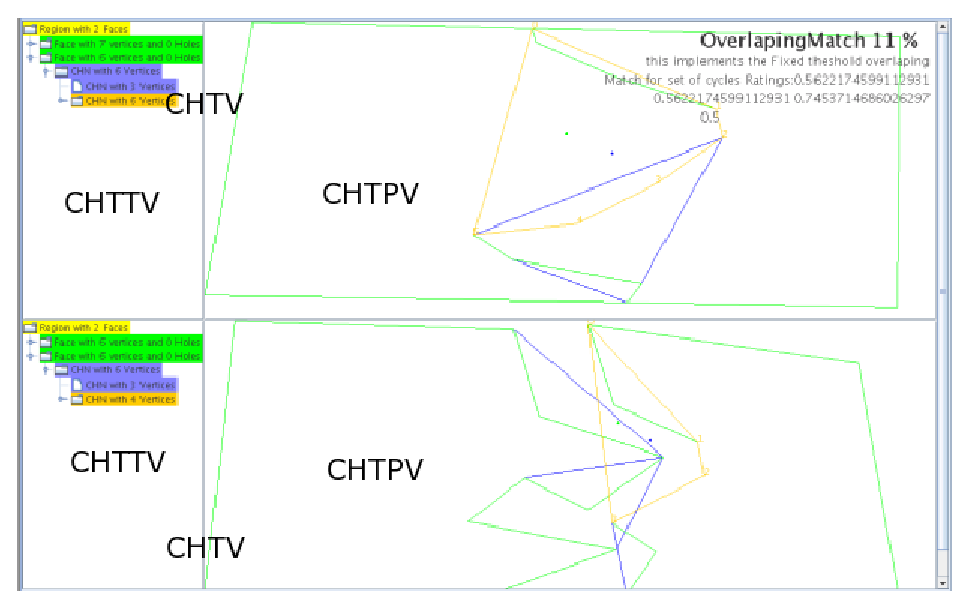
\includegraphics[scale=0.8]{MatchViewer.eps}
	\caption[Ein MatchViewer mit allen Unteklassen] {Hier sieht man die Komponenten MatchViewer, ConvexHullTreeViewer (CHTV), ConvexHullTreeTreeViewer (CHTTV) und ConvexHullPolygonViewer (CHTPV) zusammen.}
	\label{fig:MatchViewer}
\end{figure}

\item ConvexHullTreePolygonViewer

Diese Klasse dient dazu, einen RegionTree als Polygon darzustellen. Faces sind hier grün gefärbt, Holes rot und tierferliegende ConvexHullTreeNodes blau. Zu jedem ConvexHullTreeNode wird nicht nur der eigentliche Umfang des Polygons, sondern die Konvexe Hülle dargestellt.

Zusätzlich beinhaltet diese Klasse ein Attribut actual, das ein Feld von RegionTreeNodes ist. Diese Elemente werden organge dargestellt, und ermöglicht das Auswählen von Elementen, falls der ConvexHullTreePolygonViewer in einen höheren Kontext eingebunden wird.

\item ConvexHullTreeTreeViewer

Diese Klasse dient dazu, einen RegionTree als Baum darzustellen. Die Darstellung dieses Baumes orientiert sich an der Darstellung, win man sie von Verzeichnissbäumen in verschiedenen Betriebsystemen kennt.

Diese Klasse benutzt zwei Hilfsklassen:
\begin{itemize}
\item ConvexHullTreeTreeViewerNode

Diese Klasse repräsentiert einen Element des RegionTrees und kümmert sich zum einen um die textuelle Beschreibung dieses, und zum anderen darum, den Baum rekursiv aufzubauen.
\item ConvexHullTreeTreeViewerRenderer

Diese Hilfsklasse kümmert sich darum, die Darstellung der einzelnen Elemente farblich zu unterscheiden. Die Farben bei der Darstellung entsprechen denen im ConvexHullTreePolygonViewer, nur das zusätzlich noch die Farbe gelb, für das Vaterelement, die Region, benutzt wird.
\end{itemize}

Nachdem man ein Objekt dieser Klasse angelegt hat und ihm dabei den gewünschten RegionTree übergeben hat, läßt sich dieses wie jedes andere JPanel benutzen.

\item ConvexHullTreeViewer

Diese Klasse fasst die beiden Darstellungen als Baum und als Polygon zusammen. Auf der linken Seite dieser GUI-Komponente findet sich die Baum-Darstellung, und auf der rechten die Darstellung als Polygon. Die Verbindung zwischen den beiden wird hergestellt, so dass es möglich ist, in der Baumdarstellung ein, oder mehrere Nodes zu selektieren, die dann auch in der Polygondarstellung gesondert markiert werden.

\item MatchViewer

Dieses Control zeigt ein Match an, indem zwei ConvexHullTreeViewer, für die Source- und die Target-Region, übereinander dargestellt werden. Die Verbindung dieser beiden wird so umgeleitet, dass die Selektion eienes Elementes, in einem der beiden ConvexHullTreeTreeViewer die Selkektion in dem gematchten Element zu Folge hat. Konstruiert wird diese Komponente, indem man einfach ein Match übergibt. Auch diese Komponente ist von JPanel abgeleitet, und läßt sich entsprechend einsetzen.

\begin{figure}
	\centering
	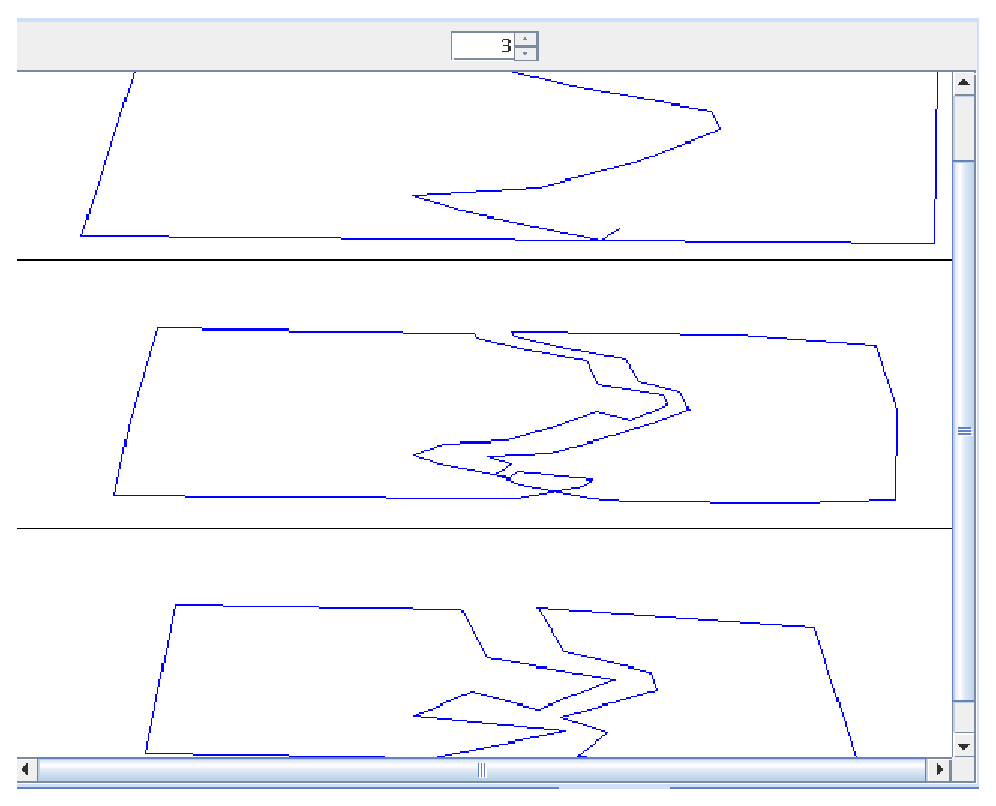
\includegraphics[scale=0.5]{Sectionviewer.eps}
	\caption{Ein SectionViewer, bestehend aus drei oneSectionViewern.}
	\label{fig:SectionViewer}
\end{figure}


\item SectionViewer

Diese Klasse stellt das Ergebniss des Matchings, die erzeugten dreidimensionalen Dreiecke dar, indem eine Menge von unterschiedlichen Schnittbildern dargestellt werden. Über ein Control läßt sich die gewünschte Anzahl der Schnittbilder einstellen und dann erscheinen diese im unteren Bereich der GUI-Komponente. Die einzelenen Schnittbilder werden von der Hilfsklasse  \textbf{oneSectionViewer} gezeichnet.

Konstruiert wird der Section-Viewer einfach, indem man diesem ein Objekt vom Typ mLineRep übergibt.


\item TriRepOutPutCanvas

Auch diese Klasse stellt ein mLineRep-Objekt dar. Allerdings erfolgt die Darstellung hier isometrisch. Die Source- und die Target-Region werden parallel zur Monitorebene dargestellt, wobei das target nach rechtsoben verschoben wird. Die Linien des Sources sind blau, die des Targets rot. Die Linien dazwischen, also die Linien der Dreiecke sind in grauer Farbe markiert.

Diese Komponente bekommt neben dem mLineRep-Objekt noch eine Ganzzahl, die den Grad der Verschiebung angibt. Diese läßt sich mittels der Methode \textbf{setTimeShift} auch nachträglich ändern. Auch wenn der Name der Klasse anderes vermuten läßt, ist diese Klasse kein Canvas sondern ein JPanel. Der Name ist noch ein Relikt von der T\o{}ssebroschen-Applikation.

\begin{figure}
	\centering
	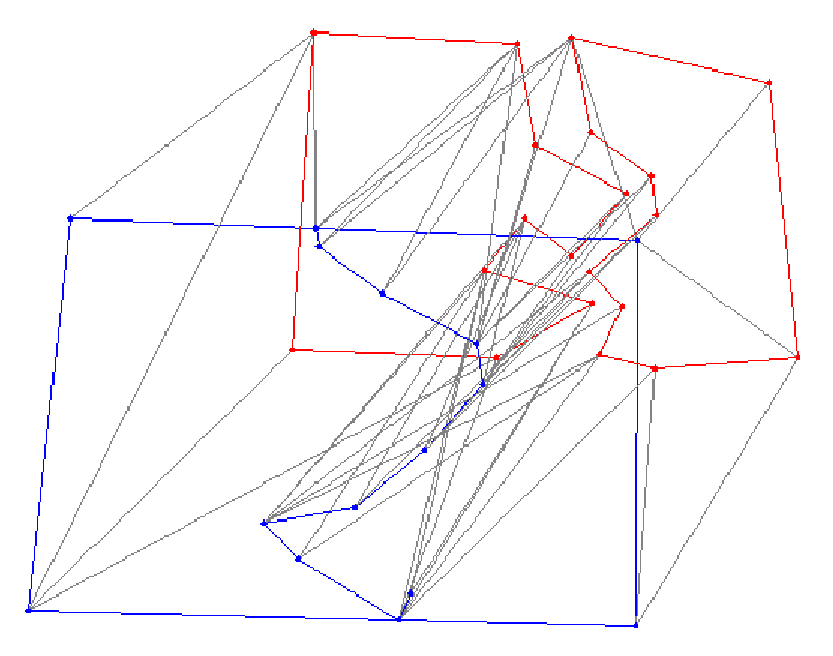
\includegraphics[scale=0.7]{TriRepOutPutCanvas.eps}
	\caption{Ein TriRepOutputCanvas.}
	\label{fig:TriRepOutputCanvas}
\end{figure}




\item tegnecanvas

Diese Klasse bildet die Zeichenfläche der Applikation. In dieser kann der Benutzer seine beiden Regionen malen. Nachdem der Benutzer dies getan hat, kann man mit den Funktionen getFirstSnapshot und getSecondSnapshot die Regionen auslesen. 

\item MCIContents

Diese Klasse vereinigt alle anderen Klassen zu der eigentlichen Applikation. Diese Klasse läßst sich entweder als Applet benutzen, oder in ein JFrame einbinden, der damit eine Standalone-Applikation bildet.
\end{itemize}
\section{Die Secondo-Algebra \anmerkung{3 Seiten}}\label{rialgebra}
\anmerkung{Hier beschreibe ich kurz, wie ich die Secondo-Algebra implementiert habe. Speziell die Einbettung in das Secondo soll hier betrachtet werden.}

\subsection{MovingRegionAlgebra}

\subsection{PlaneSweepAlgebra}

\subsection{SpatialAlgebra}

\subsection{RegionInterpolationAlgebra}

